% -----------------------------------------------------------------------------
%                                     HEADER                                    
% -----------------------------------------------------------------------------
\documentclass[a4paper, 10pt]{article}
\usepackage{jheppub}
\usepackage[T1]{fontenc}
\usepackage{colortbl,xcolor,float}
\definecolor{orange}{rgb}{1,0.5,0}
% -----------------------------------------------------------------------------
%                                   COVER PAGE                                  
% -----------------------------------------------------------------------------
\title{{
\includegraphics[scale=.4]{logo.eps}}\ The LaTeX report}

\author{Generated by s1412595 on 08 July 2019, 15:57:18}

\abstract{
  This report has been generated automatically
  by {\sc MadAnalysis} 5.\\$~$\\ 
  Please cite:\\ 
  \begin{quote}
    \textbf{E.~Conte, B.~Fuks and G.~Serret},\\ 
    \textit{MadAnalysis 5, A User-Friendly
    Framework for Collider Phenomenology},\\ 
    Comput. Phys. Commun. {\bf 184} (2013) 222-256,\\
    arXiv:1206.1599 [hep-ph].\\ 
  \end{quote}
  To contact us:\\ 
  \begin{quote}
    \textbf{http://madanalysis.irmp.ucl.ac.be}\\
    \textbf{ma5team@iphc.cnrs.fr}\\
  \end{quote}
}

% -----------------------------------------------------------------------------
%                                 BEGIN DOCUMENT                                
% -----------------------------------------------------------------------------
\begin{document}
\maketitle
\flushbottom

% -----------------------------------------------------------------------------
%                                 SECTION Setup                                 
% -----------------------------------------------------------------------------
\newpage
\section{ Setup}

\subsection{ Command history}

\texttt{ma5>define invisible = 12 14 16 -12 -14 -16\\
}
\texttt{ }\texttt{ }\texttt{ma5>set main.fastsim.package = fastjet\\
}
\texttt{ }\texttt{ }\texttt{ma5>set main.fastsim.algorithm = antikt\\
}
\texttt{ }\texttt{ }\texttt{ma5>set main.fastsim.radius = 0.4\\
}
\texttt{ }\texttt{ }\texttt{ma5>set main.fastsim.ptmin = 5.0\\
}
\texttt{ }\texttt{ }\texttt{ma5>set main.fastsim.bjet\_id.matching\_dr = 0.4\\
}
\texttt{ }\texttt{ }\texttt{ma5>set main.fastsim.bjet\_id.efficiency = 1.0\\
}
\texttt{ }\texttt{ }\texttt{ma5>set main.fastsim.bjet\_id.misid\_cjet = 0.0\\
}
\texttt{ }\texttt{ }\texttt{ma5>set main.fastsim.bjet\_id.misid\_ljet = 0.0\\
}
\texttt{ }\texttt{ }\texttt{ma5>set main.fastsim.tau\_id.efficiency = 1.0\\
}
\texttt{ }\texttt{ }\texttt{ma5>set main.fastsim.tau\_id.misid\_ljet = 0.0\\
}
\texttt{ }\texttt{ }\texttt{ma5>import /\-home/\-s1412595/\-Desktop/\-SummerProject2019/\-MG5\_aMC\_v2\_6\_6/\-BP2\_080719/\-Events/\-run\_01/\-tag\_1\_pythia8\_events.hepmc.gz as reco\_events\\
}
\texttt{ }\texttt{ }\texttt{ma5>set main.outputfile=tag\_1\_pythia8\_BasicReco.lhe.gz\\
}
\texttt{ }\texttt{ }\texttt{ma5>submit /\-home/\-s1412595/\-Desktop/\-SummerProject2019/\-MG5\_aMC\_v2\_6\_6/\-BP2\_080719/\-MA5\_HADRON\_ANALYSIS\_reco\_BasicReco\_1\\
}
\texttt{ }\texttt{ }\texttt{ma5>remove reco\_events\\
}
\texttt{ }\texttt{ }\texttt{ma5>set main.mode = parton\\
}
\texttt{ }\texttt{ }\texttt{ma5>import /\-home/\-s1412595/\-Desktop/\-SummerProject2019/\-MG5\_aMC\_v2\_6\_6/\-BP2\_080719/\-Events/\-run\_01/\-tag\_1\_pythia8\_BasicReco.lhe.gz as tag\_1\_pythia8\_BasicReco\\
}
\texttt{ }\texttt{ }\texttt{ma5>set main.stacking\_method = normalize2one\\
}
\texttt{ }\texttt{ }\texttt{ma5>define e = e+ e-\\
}
\texttt{ }\texttt{ }\texttt{ma5>define mu = mu+ mu-\\
}
\texttt{ }\texttt{ }\texttt{ma5>select (j)  PT > 20\\
}
\texttt{ }\texttt{ }\texttt{ma5>select (b)  PT > 20\\
}
\texttt{ }\texttt{ }\texttt{ma5>select (e)  PT > 10\\
}
\texttt{ }\texttt{ }\texttt{ma5>select (mu) PT > 10\\
}
\texttt{ }\texttt{ }\texttt{ma5>select (j)  ABSETA < 2.5\\
}
\texttt{ }\texttt{ }\texttt{ma5>select (b)  ABSETA < 2.5\\
}
\texttt{ }\texttt{ }\texttt{ma5>select (e)  ABSETA < 2.5\\
}
\texttt{ }\texttt{ }\texttt{ma5>select (mu) ABSETA < 2.5\\
}
\texttt{ }\texttt{ }\texttt{ma5>plot MET 40 0 500\\
}
\texttt{ }\texttt{ }\texttt{ma5>plot THT 40 0 500\\
}
\texttt{ }\texttt{ }\texttt{ma5>plot PT(j[1]) 40 0 500 [logY]\\
}
\texttt{ }\texttt{ }\texttt{ma5>plot ETA(j[1]) 40 -10 10 [logY]\\
}
\texttt{ }\texttt{ }\texttt{ma5>plot MT\_MET(j[1]) 40 0 500 [logY]\\
}
\texttt{ }\texttt{ }\texttt{ma5>plot PT(j[2]) 40 0 500 [logY]\\
}
\texttt{ }\texttt{ }\texttt{ma5>plot ETA(j[2]) 40 -10 10 [logY]\\
}
\texttt{ }\texttt{ }\texttt{ma5>plot MT\_MET(j[2]) 40 0 500 [logY]\\
}
\texttt{ }\texttt{ }\texttt{ma5>plot PT(e[1]) 40 0 500 [logY]\\
}
\texttt{ }\texttt{ }\texttt{ma5>plot ETA(e[1]) 40 -10 10 [logY]\\
}
\texttt{ }\texttt{ }\texttt{ma5>plot MT\_MET(e[1]) 40 0 500 [logY]\\
}
\texttt{ }\texttt{ }\texttt{ma5>plot PT(mu[1]) 40 0 500 [logY]\\
}
\texttt{ }\texttt{ }\texttt{ma5>plot ETA(mu[1]) 40 -10 10 [logY]\\
}
\texttt{ }\texttt{ }\texttt{ma5>plot MT\_MET(mu[1]) 40 0 500 [logY]\\
}
\texttt{ }\texttt{ }\texttt{ma5>plot M(e[1] mu[1]) 40 0  500 [logY]\\
}
\texttt{ }\texttt{ }\texttt{ma5>plot M(j[1] e[1]) 40 0  500 [logY]\\
}
\texttt{ }\texttt{ }\texttt{ma5>plot M(j[1] j[2]) 40 0  500 [logY]\\
}
\texttt{ }\texttt{ }\texttt{ma5>plot M(j[1] mu[1]) 40 0  500 [logY]\\
}
\texttt{ }\texttt{ }\texttt{ma5>plot M(j[2] e[1]) 40 0  500 [logY]\\
}
\texttt{ }\texttt{ }\texttt{ma5>plot M(j[2] mu[1]) 40 0  500 [logY]\\
}
\texttt{ }\texttt{ }\texttt{ma5>plot DELTAR(e[1],mu[1]) 40 0 10 [logY]\\
}
\texttt{ }\texttt{ }\texttt{ma5>plot DELTAR(j[1],e[1]) 40 0 10 [logY]\\
}
\texttt{ }\texttt{ }\texttt{ma5>plot DELTAR(j[1],j[2]) 40 0 10 [logY]\\
}
\texttt{ }\texttt{ }\texttt{ma5>plot DELTAR(j[1],mu[1]) 40 0 10 [logY]\\
}
\texttt{ }\texttt{ }\texttt{ma5>plot DELTAR(j[2],e[1]) 40 0 10 [logY]\\
}
\texttt{ }\texttt{ }\texttt{ma5>plot DELTAR(j[2],mu[1]) 40 0 10 [logY]\\
}
\texttt{ }\texttt{ }\texttt{ma5>submit /\-home/\-s1412595/\-Desktop/\-SummerProject2019/\-MG5\_aMC\_v2\_6\_6/\-BP2\_080719/\-MA5\_HADRON\_ANALYSIS\_analysis2\_BasicReco\\
}
\texttt{ }\texttt{ }\subsection{ Configuration}

\begin{itemize}
  \item MadAnalysis version 1.8.5 (2019/\-04/\-04).
   \item Histograms given for an integrated luminosity of \textcolor{blue}{10}\textcolor{blue}{ fb}$^{\textcolor{blue}{-1}}$\textcolor{blue}{.}
\textcolor{blue}{}
\end{itemize}
% -----------------------------------------------------------------------------
%                                SECTION Datasets                               
% -----------------------------------------------------------------------------
\newpage
\section{ Datasets}

\subsection{ tag\_1\_pythia8\_basicreco}

\begin{itemize}
  \item Sample consisting of: \textcolor{blue}{signal}  events.
   \item Generated events: \textcolor{blue}{1000 }  events.
   \item Normalization to the luminosity: \textcolor{blue}{0}\textcolor{blue}{ +/\-- }\textcolor{blue}{0 }  events.
   \item Ratio (event weight): \textcolor{blue}{0.0 } .  
 
\end{itemize}
\begin{table}[H]
  \begin{center}
    \begin{tabular}{|m{55.0mm}|m{25.0mm}|m{30.0mm}|m{30.0mm}|}
      \hline
      {\cellcolor{yellow}         Path to the event file}& {\cellcolor{yellow}         Nr. of events}& {\cellcolor{yellow}         Cross section (pb)}& {\cellcolor{yellow}         Negative wgts (\%)}\\
      \hline
      {\cellcolor{white}          Events/\-run\_01/\-tag\_1\_pythia8\_BasicReco.lhe.gz}& {\cellcolor{white}          1000}& {\cellcolor{white}          0.0 @ 0.0\%}& {\cellcolor{white}          0.0}\\
\hline
    \end{tabular}
  \end{center}
\end{table}

% -----------------------------------------------------------------------------
%                            SECTION Histos and cuts                            
% -----------------------------------------------------------------------------
\newpage
\section{ Histos and cuts}

\subsection{ Object definition 1}

\textbf{* Cut: select ( j ) PT > 20.0}\\
   \subsection{ Object definition 2}

\textbf{* Cut: select ( b ) PT > 20.0}\\
   \subsection{ Object definition 3}

\textbf{* Cut: select ( e ) PT > 10.0}\\
   \subsection{ Object definition 4}

\textbf{* Cut: select ( mu ) PT > 10.0}\\
   \subsection{ Object definition 5}

\textbf{* Cut: select ( j ) ABSETA < 2.5}\\
   \subsection{ Object definition 6}

\textbf{* Cut: select ( b ) ABSETA < 2.5}\\
   \subsection{ Object definition 7}

\textbf{* Cut: select ( e ) ABSETA < 2.5}\\
   \subsection{ Object definition 8}

\textbf{* Cut: select ( mu ) ABSETA < 2.5}\\
   \subsection{ Histogram 1}

\textbf{* Plot: MET}\\
   \begin{table}[H]
  \begin{center}
    \begin{tabular}{|m{23.0mm}|m{23.0mm}|m{18.0mm}|m{19.0mm}|m{19.0mm}|m{19.0mm}|m{19.0mm}|}
      \hline
      {\cellcolor{yellow}         Dataset}& {\cellcolor{yellow}         Integral}& {\cellcolor{yellow}         Entries per event}& {\cellcolor{yellow}         Mean}& {\cellcolor{yellow}         RMS}& {\cellcolor{yellow}         \% underflow}& {\cellcolor{yellow}         \% overflow}\\
      \hline
      {\cellcolor{white}         tag\_1\_pythia8\_basicreco}& {\cellcolor{white}         0.0 +/\-- 0.0}& {\cellcolor{white}         1.0}& {\cellcolor{white}         0.0}& {\cellcolor{white}         0.0}& {\cellcolor{green}         0.0}& {\cellcolor{green}         0.0}\\
\hline
    \end{tabular}
  \end{center}
\end{table}

\begin{figure}[H]
  \begin{center}
    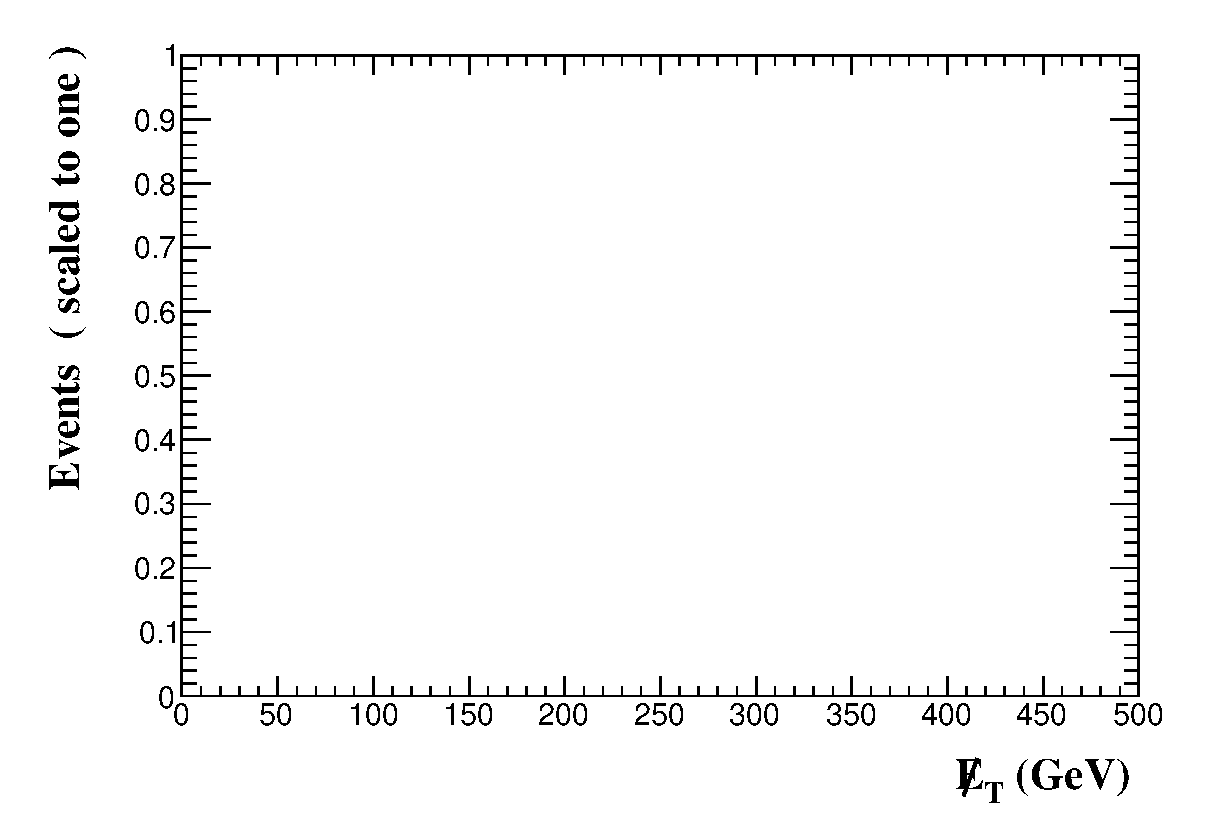
\includegraphics[scale=0.45]{selection_0.eps}\\
\caption{   }
  \end{center}
\end{figure}
      \newpage
\subsection{ Histogram 2}

\textbf{* Plot: THT}\\
   \begin{table}[H]
  \begin{center}
    \begin{tabular}{|m{23.0mm}|m{23.0mm}|m{18.0mm}|m{19.0mm}|m{19.0mm}|m{19.0mm}|m{19.0mm}|}
      \hline
      {\cellcolor{yellow}         Dataset}& {\cellcolor{yellow}         Integral}& {\cellcolor{yellow}         Entries per event}& {\cellcolor{yellow}         Mean}& {\cellcolor{yellow}         RMS}& {\cellcolor{yellow}         \% underflow}& {\cellcolor{yellow}         \% overflow}\\
      \hline
      {\cellcolor{white}         tag\_1\_pythia8\_basicreco}& {\cellcolor{white}         0.0 +/\-- 0.0}& {\cellcolor{white}         1.0}& {\cellcolor{white}         0.0}& {\cellcolor{white}         0.0}& {\cellcolor{green}         0.0}& {\cellcolor{green}         0.0}\\
\hline
    \end{tabular}
  \end{center}
\end{table}

\begin{figure}[H]
  \begin{center}
    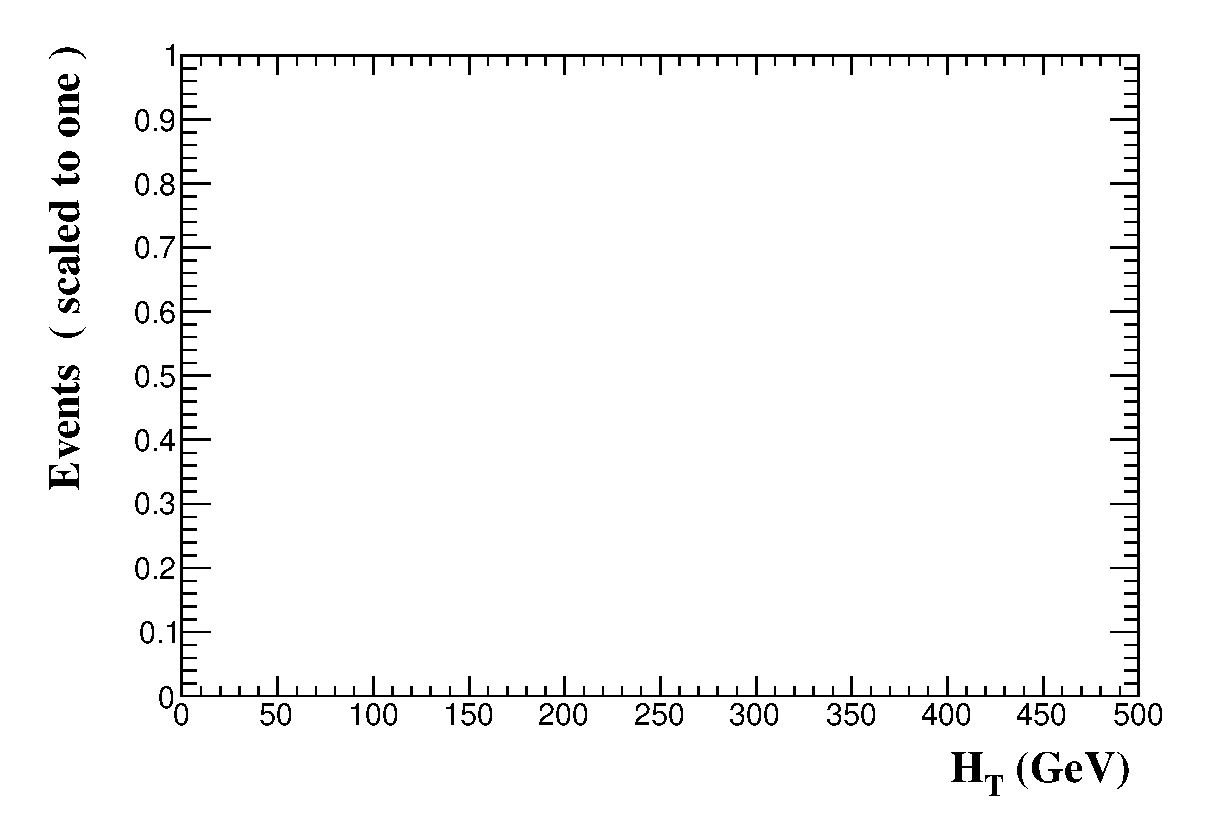
\includegraphics[scale=0.45]{selection_1.eps}\\
\caption{   }
  \end{center}
\end{figure}
      \newpage
\subsection{ Histogram 3}

\textbf{* Plot: PT ( j[1] ) }\\
   \begin{table}[H]
  \begin{center}
    \begin{tabular}{|m{23.0mm}|m{23.0mm}|m{18.0mm}|m{19.0mm}|m{19.0mm}|m{19.0mm}|m{19.0mm}|}
      \hline
      {\cellcolor{yellow}         Dataset}& {\cellcolor{yellow}         Integral}& {\cellcolor{yellow}         Entries per event}& {\cellcolor{yellow}         Mean}& {\cellcolor{yellow}         RMS}& {\cellcolor{yellow}         \% underflow}& {\cellcolor{yellow}         \% overflow}\\
      \hline
      {\cellcolor{white}         tag\_1\_pythia8\_basicreco}& {\cellcolor{white}         0.0 +/\-- 0.0}& {\cellcolor{white}         1.0}& {\cellcolor{white}         0.0}& {\cellcolor{white}         0.0}& {\cellcolor{green}         0.0}& {\cellcolor{green}         0.0}\\
\hline
    \end{tabular}
  \end{center}
\end{table}

\begin{figure}[H]
  \begin{center}
    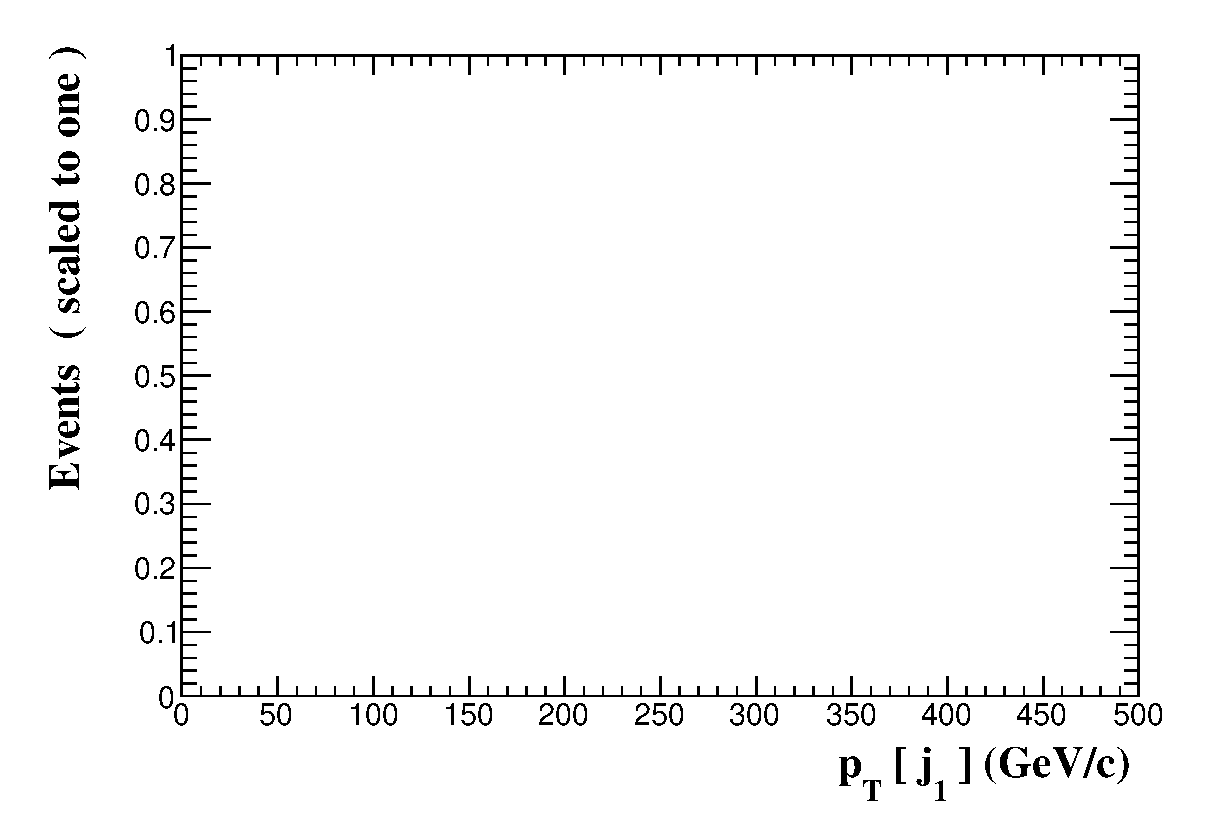
\includegraphics[scale=0.45]{selection_2.eps}\\
\caption{   }
  \end{center}
\end{figure}
      \newpage
\subsection{ Histogram 4}

\textbf{* Plot: ETA ( j[1] ) }\\
   \begin{table}[H]
  \begin{center}
    \begin{tabular}{|m{23.0mm}|m{23.0mm}|m{18.0mm}|m{19.0mm}|m{19.0mm}|m{19.0mm}|m{19.0mm}|}
      \hline
      {\cellcolor{yellow}         Dataset}& {\cellcolor{yellow}         Integral}& {\cellcolor{yellow}         Entries per event}& {\cellcolor{yellow}         Mean}& {\cellcolor{yellow}         RMS}& {\cellcolor{yellow}         \% underflow}& {\cellcolor{yellow}         \% overflow}\\
      \hline
      {\cellcolor{white}         tag\_1\_pythia8\_basicreco}& {\cellcolor{white}         0.0 +/\-- 0.0}& {\cellcolor{white}         1.0}& {\cellcolor{white}         0.0}& {\cellcolor{white}         0.0}& {\cellcolor{green}         0.0}& {\cellcolor{green}         0.0}\\
\hline
    \end{tabular}
  \end{center}
\end{table}

\begin{figure}[H]
  \begin{center}
    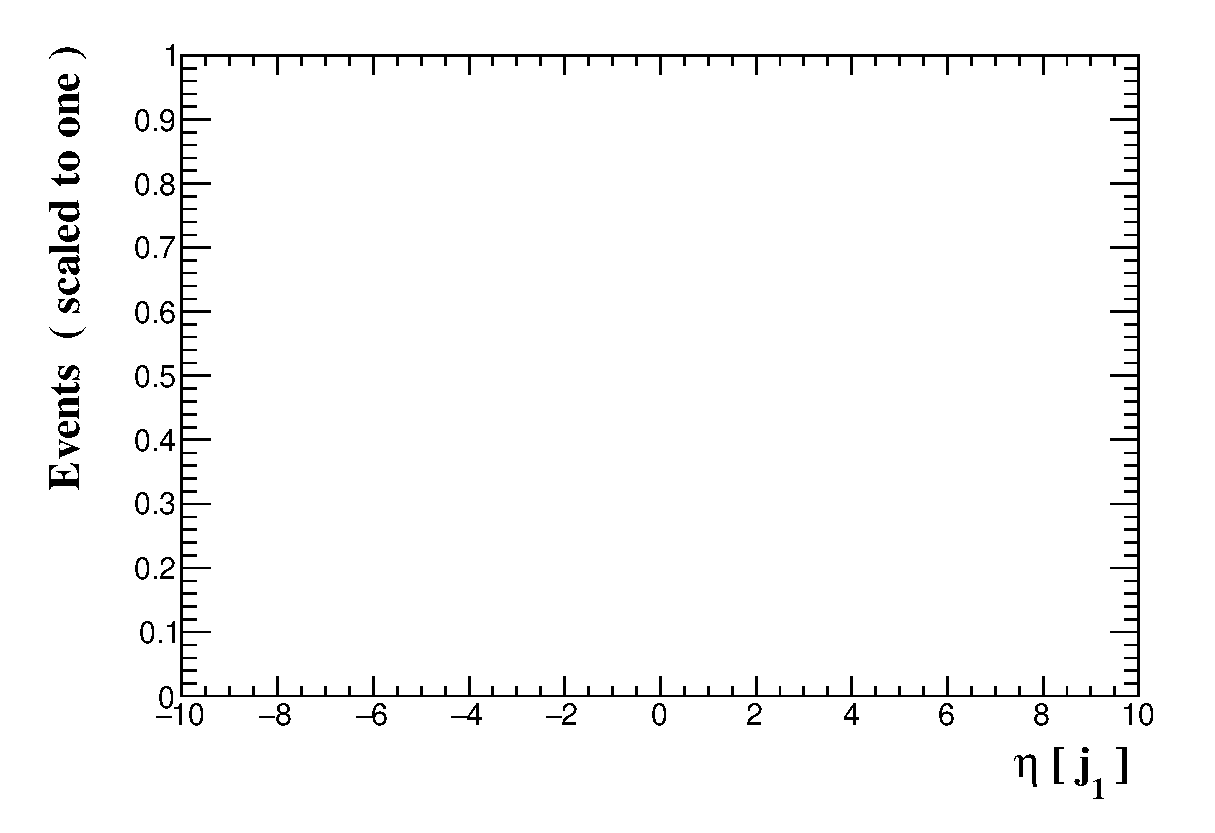
\includegraphics[scale=0.45]{selection_3.eps}\\
\caption{   }
  \end{center}
\end{figure}
      \newpage
\subsection{ Histogram 5}

\textbf{* Plot: MT\_MET ( j[1] ) }\\
   \begin{table}[H]
  \begin{center}
    \begin{tabular}{|m{23.0mm}|m{23.0mm}|m{18.0mm}|m{19.0mm}|m{19.0mm}|m{19.0mm}|m{19.0mm}|}
      \hline
      {\cellcolor{yellow}         Dataset}& {\cellcolor{yellow}         Integral}& {\cellcolor{yellow}         Entries per event}& {\cellcolor{yellow}         Mean}& {\cellcolor{yellow}         RMS}& {\cellcolor{yellow}         \% underflow}& {\cellcolor{yellow}         \% overflow}\\
      \hline
      {\cellcolor{white}         tag\_1\_pythia8\_basicreco}& {\cellcolor{white}         0.0 +/\-- 0.0}& {\cellcolor{white}         1.0}& {\cellcolor{white}         0.0}& {\cellcolor{white}         0.0}& {\cellcolor{green}         0.0}& {\cellcolor{green}         0.0}\\
\hline
    \end{tabular}
  \end{center}
\end{table}

\begin{figure}[H]
  \begin{center}
    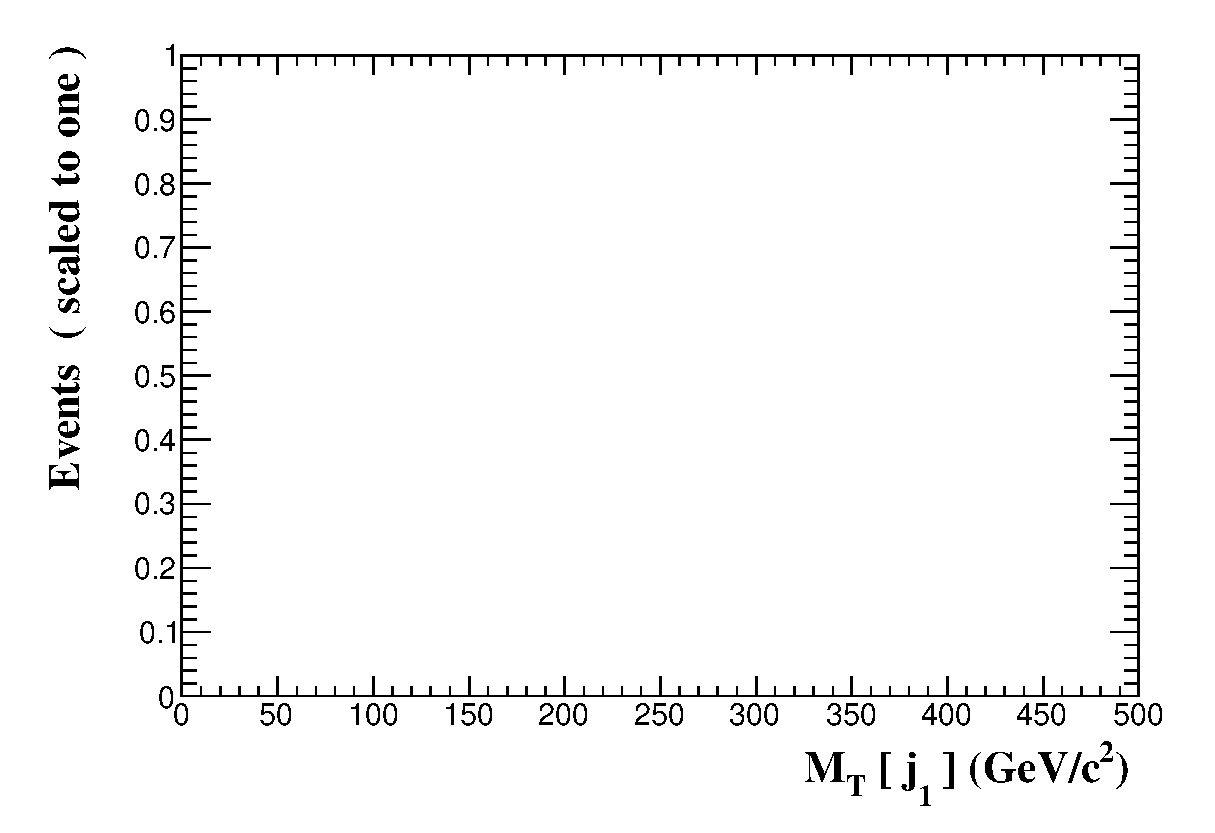
\includegraphics[scale=0.45]{selection_4.eps}\\
\caption{   }
  \end{center}
\end{figure}
      \newpage
\subsection{ Histogram 6}

\textbf{* Plot: PT ( j[2] ) }\\
   \begin{table}[H]
  \begin{center}
    \begin{tabular}{|m{23.0mm}|m{23.0mm}|m{18.0mm}|m{19.0mm}|m{19.0mm}|m{19.0mm}|m{19.0mm}|}
      \hline
      {\cellcolor{yellow}         Dataset}& {\cellcolor{yellow}         Integral}& {\cellcolor{yellow}         Entries per event}& {\cellcolor{yellow}         Mean}& {\cellcolor{yellow}         RMS}& {\cellcolor{yellow}         \% underflow}& {\cellcolor{yellow}         \% overflow}\\
      \hline
      {\cellcolor{white}         tag\_1\_pythia8\_basicreco}& {\cellcolor{white}         0.0 +/\-- 0.0}& {\cellcolor{white}         1.0}& {\cellcolor{white}         0.0}& {\cellcolor{white}         0.0}& {\cellcolor{green}         0.0}& {\cellcolor{green}         0.0}\\
\hline
    \end{tabular}
  \end{center}
\end{table}

\begin{figure}[H]
  \begin{center}
    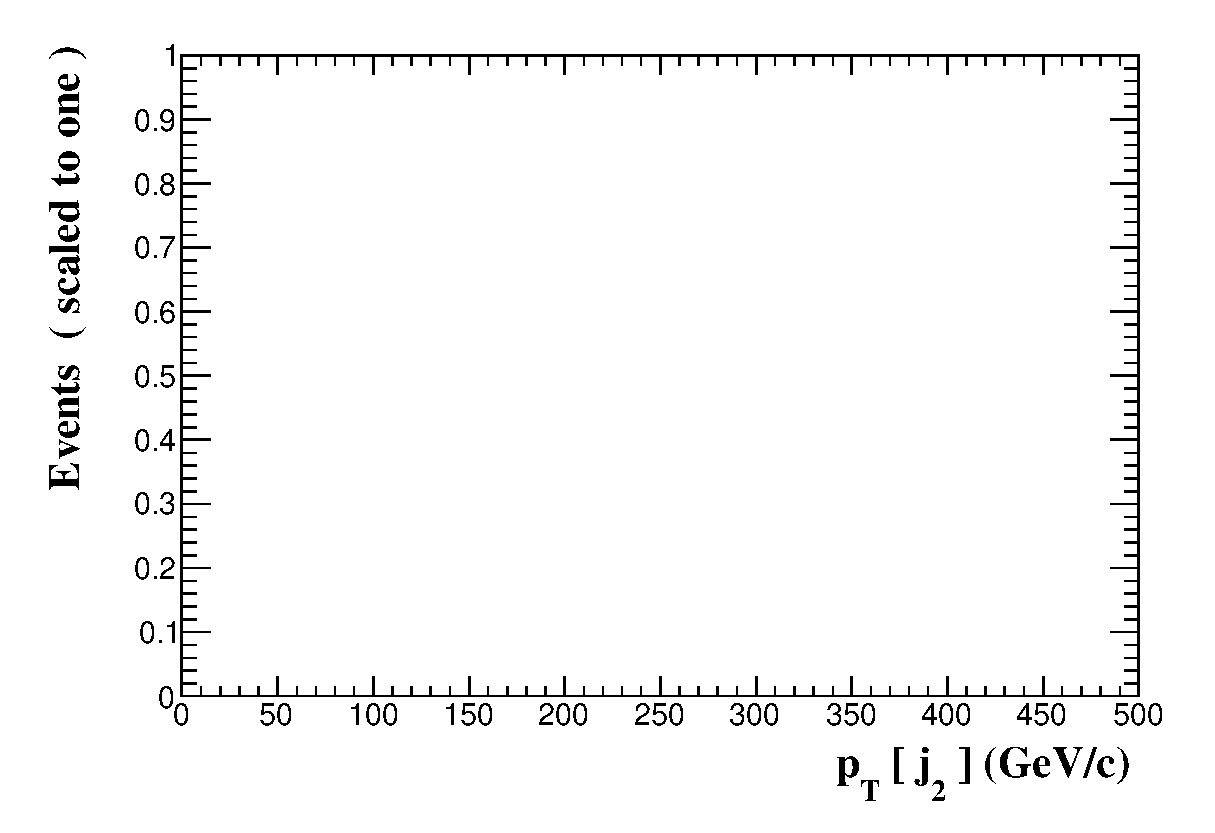
\includegraphics[scale=0.45]{selection_5.eps}\\
\caption{   }
  \end{center}
\end{figure}
      \newpage
\subsection{ Histogram 7}

\textbf{* Plot: ETA ( j[2] ) }\\
   \begin{table}[H]
  \begin{center}
    \begin{tabular}{|m{23.0mm}|m{23.0mm}|m{18.0mm}|m{19.0mm}|m{19.0mm}|m{19.0mm}|m{19.0mm}|}
      \hline
      {\cellcolor{yellow}         Dataset}& {\cellcolor{yellow}         Integral}& {\cellcolor{yellow}         Entries per event}& {\cellcolor{yellow}         Mean}& {\cellcolor{yellow}         RMS}& {\cellcolor{yellow}         \% underflow}& {\cellcolor{yellow}         \% overflow}\\
      \hline
      {\cellcolor{white}         tag\_1\_pythia8\_basicreco}& {\cellcolor{white}         0.0 +/\-- 0.0}& {\cellcolor{white}         1.0}& {\cellcolor{white}         0.0}& {\cellcolor{white}         0.0}& {\cellcolor{green}         0.0}& {\cellcolor{green}         0.0}\\
\hline
    \end{tabular}
  \end{center}
\end{table}

\begin{figure}[H]
  \begin{center}
    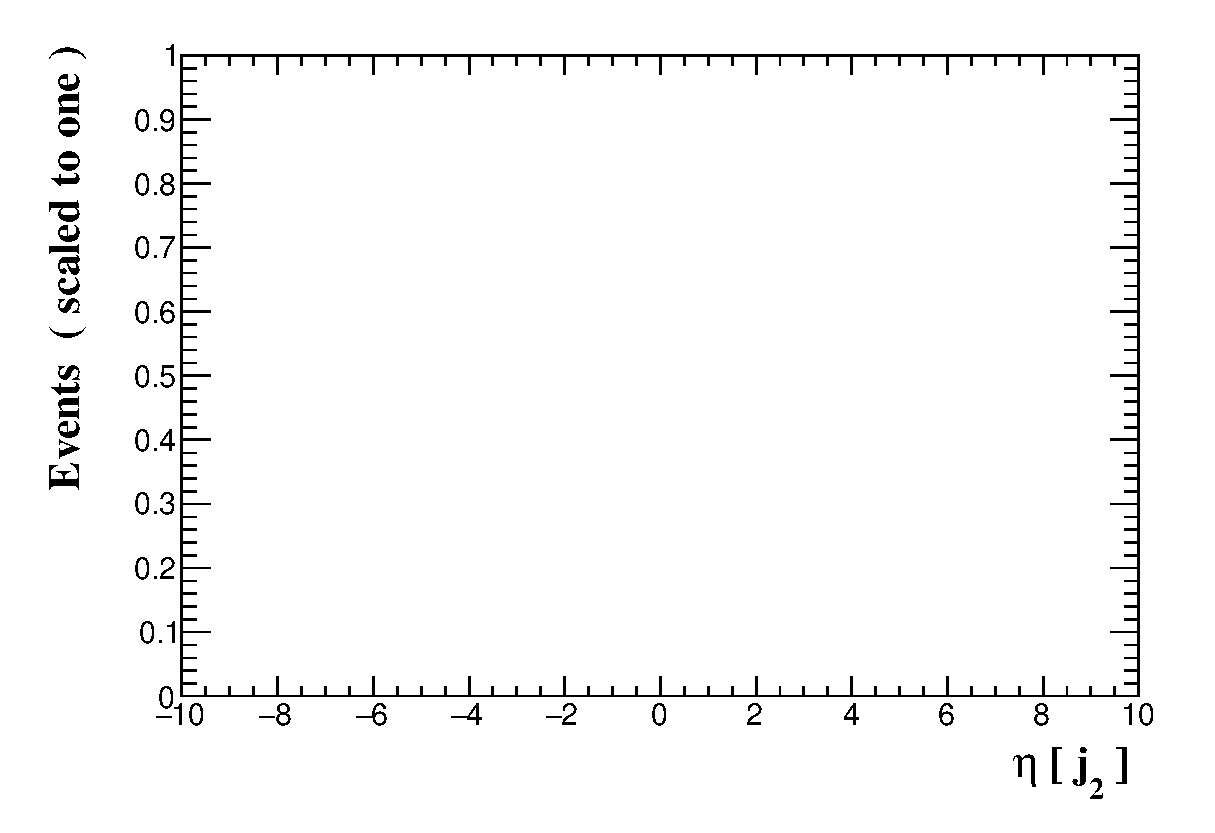
\includegraphics[scale=0.45]{selection_6.eps}\\
\caption{   }
  \end{center}
\end{figure}
      \newpage
\subsection{ Histogram 8}

\textbf{* Plot: MT\_MET ( j[2] ) }\\
   \begin{table}[H]
  \begin{center}
    \begin{tabular}{|m{23.0mm}|m{23.0mm}|m{18.0mm}|m{19.0mm}|m{19.0mm}|m{19.0mm}|m{19.0mm}|}
      \hline
      {\cellcolor{yellow}         Dataset}& {\cellcolor{yellow}         Integral}& {\cellcolor{yellow}         Entries per event}& {\cellcolor{yellow}         Mean}& {\cellcolor{yellow}         RMS}& {\cellcolor{yellow}         \% underflow}& {\cellcolor{yellow}         \% overflow}\\
      \hline
      {\cellcolor{white}         tag\_1\_pythia8\_basicreco}& {\cellcolor{white}         0.0 +/\-- 0.0}& {\cellcolor{white}         1.0}& {\cellcolor{white}         0.0}& {\cellcolor{white}         0.0}& {\cellcolor{green}         0.0}& {\cellcolor{green}         0.0}\\
\hline
    \end{tabular}
  \end{center}
\end{table}

\begin{figure}[H]
  \begin{center}
    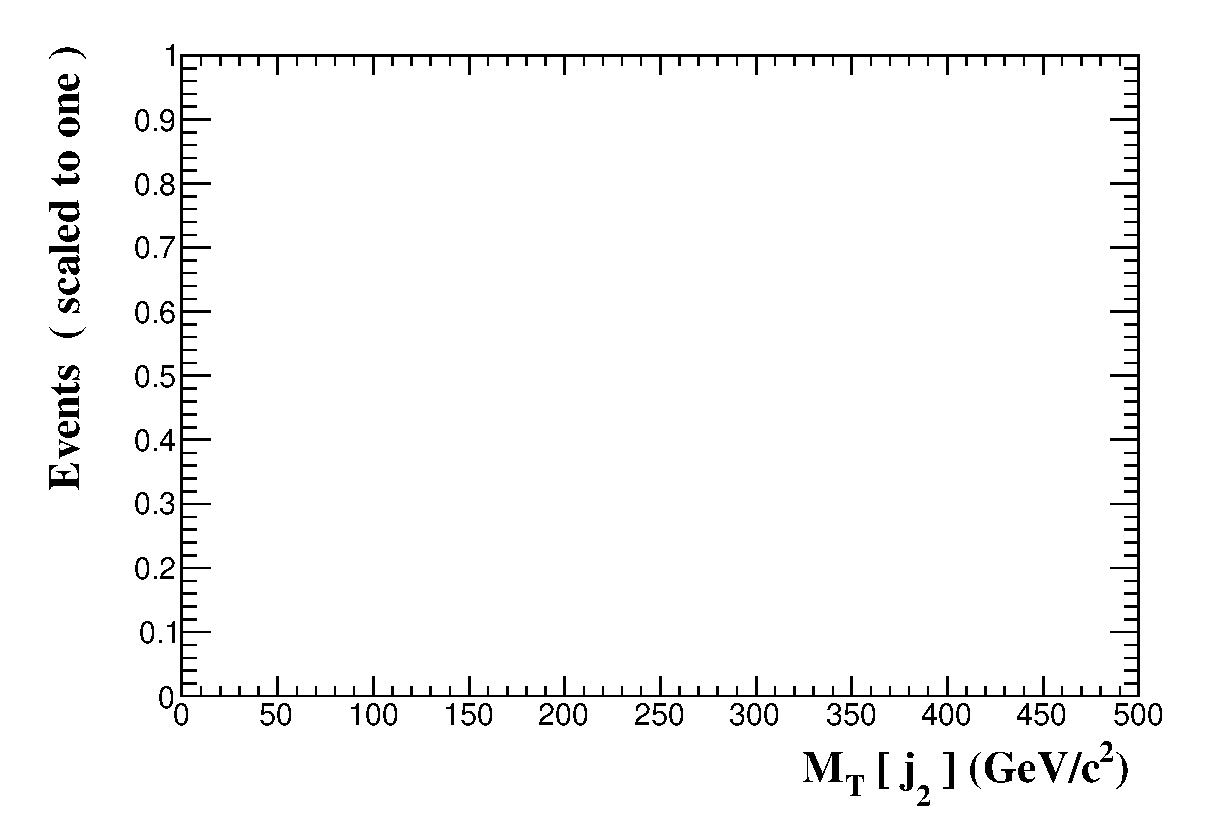
\includegraphics[scale=0.45]{selection_7.eps}\\
\caption{   }
  \end{center}
\end{figure}
      \newpage
\subsection{ Histogram 9}

\textbf{* Plot: PT ( e[1] ) }\\
   \begin{table}[H]
  \begin{center}
    \begin{tabular}{|m{23.0mm}|m{23.0mm}|m{18.0mm}|m{19.0mm}|m{19.0mm}|m{19.0mm}|m{19.0mm}|}
      \hline
      {\cellcolor{yellow}         Dataset}& {\cellcolor{yellow}         Integral}& {\cellcolor{yellow}         Entries per event}& {\cellcolor{yellow}         Mean}& {\cellcolor{yellow}         RMS}& {\cellcolor{yellow}         \% underflow}& {\cellcolor{yellow}         \% overflow}\\
      \hline
      {\cellcolor{white}         tag\_1\_pythia8\_basicreco}& {\cellcolor{white}         0.0 +/\-- 0.0}& {\cellcolor{white}         1.0}& {\cellcolor{white}         0.0}& {\cellcolor{white}         0.0}& {\cellcolor{green}         0.0}& {\cellcolor{green}         0.0}\\
\hline
    \end{tabular}
  \end{center}
\end{table}

\begin{figure}[H]
  \begin{center}
    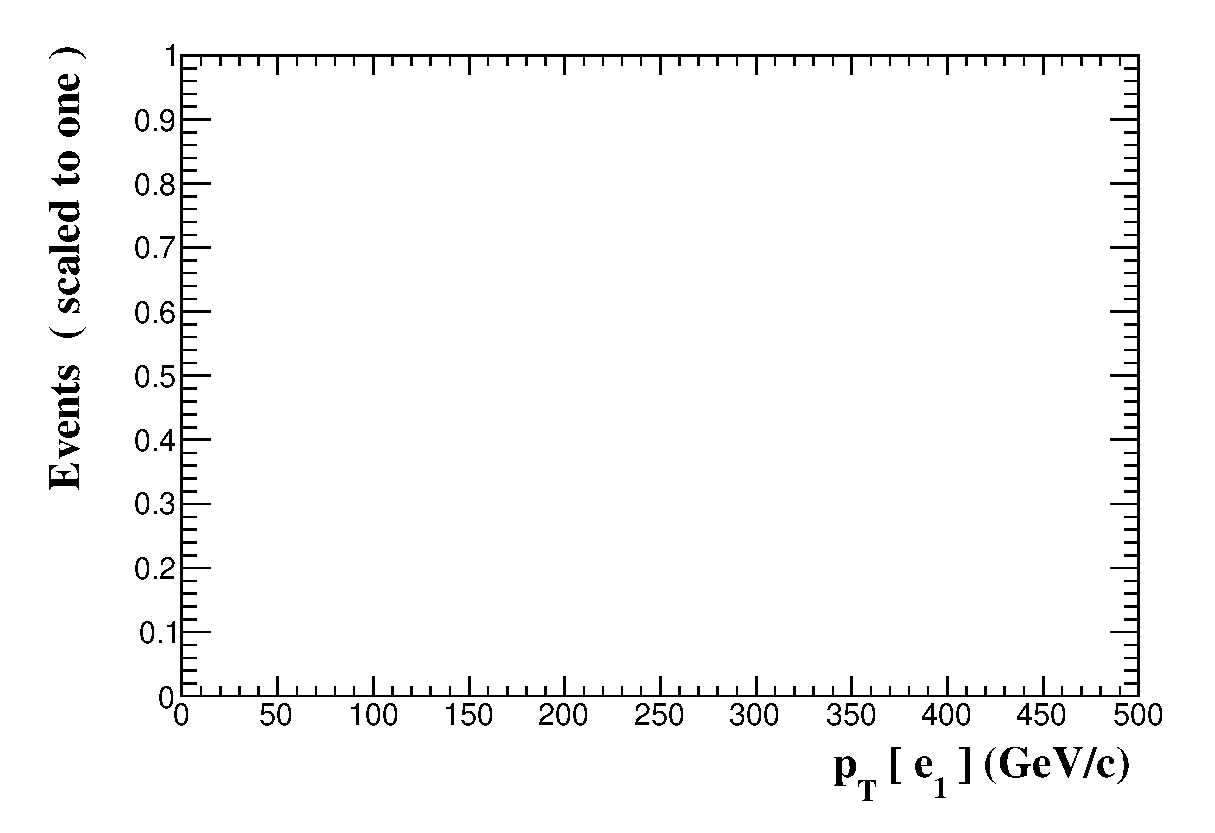
\includegraphics[scale=0.45]{selection_8.eps}\\
\caption{   }
  \end{center}
\end{figure}
      \newpage
\subsection{ Histogram 10}

\textbf{* Plot: ETA ( e[1] ) }\\
   \begin{table}[H]
  \begin{center}
    \begin{tabular}{|m{23.0mm}|m{23.0mm}|m{18.0mm}|m{19.0mm}|m{19.0mm}|m{19.0mm}|m{19.0mm}|}
      \hline
      {\cellcolor{yellow}         Dataset}& {\cellcolor{yellow}         Integral}& {\cellcolor{yellow}         Entries per event}& {\cellcolor{yellow}         Mean}& {\cellcolor{yellow}         RMS}& {\cellcolor{yellow}         \% underflow}& {\cellcolor{yellow}         \% overflow}\\
      \hline
      {\cellcolor{white}         tag\_1\_pythia8\_basicreco}& {\cellcolor{white}         0.0 +/\-- 0.0}& {\cellcolor{white}         1.0}& {\cellcolor{white}         0.0}& {\cellcolor{white}         0.0}& {\cellcolor{green}         0.0}& {\cellcolor{green}         0.0}\\
\hline
    \end{tabular}
  \end{center}
\end{table}

\begin{figure}[H]
  \begin{center}
    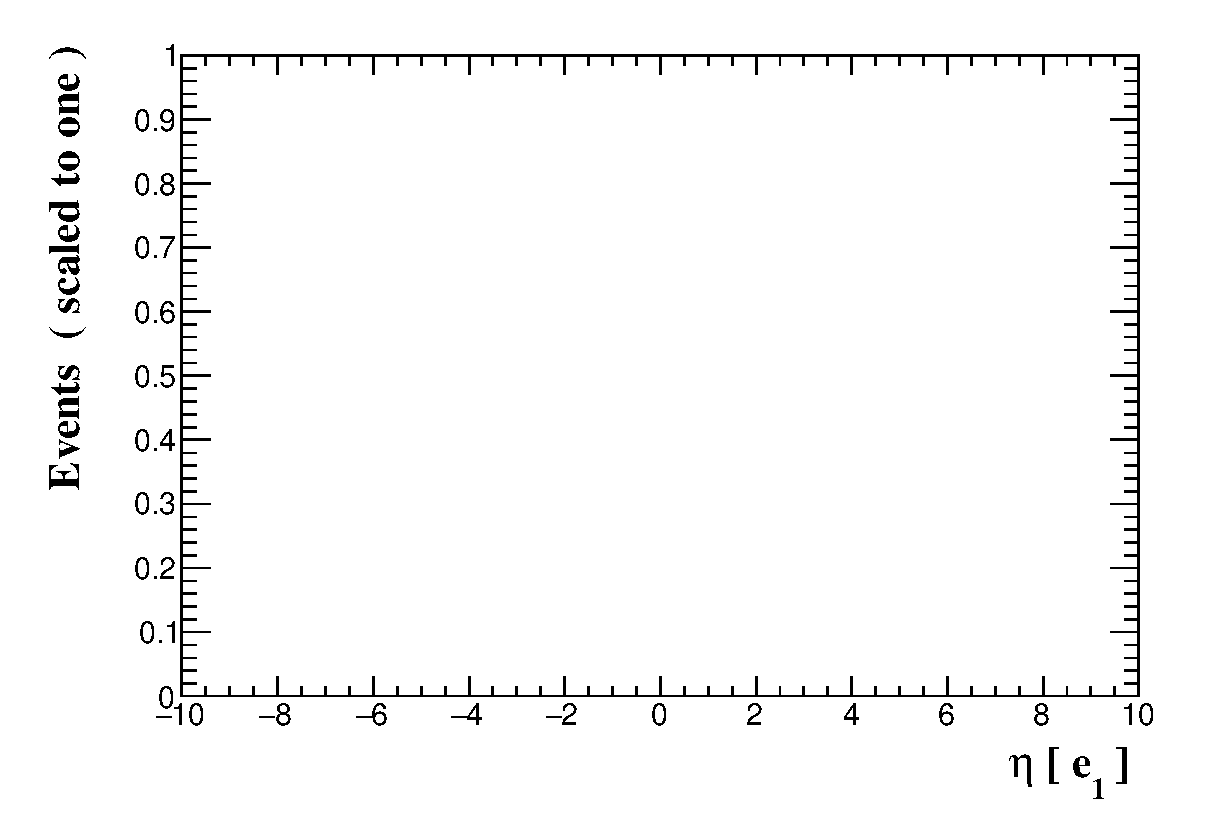
\includegraphics[scale=0.45]{selection_9.eps}\\
\caption{   }
  \end{center}
\end{figure}
      \newpage
\subsection{ Histogram 11}

\textbf{* Plot: MT\_MET ( e[1] ) }\\
   \begin{table}[H]
  \begin{center}
    \begin{tabular}{|m{23.0mm}|m{23.0mm}|m{18.0mm}|m{19.0mm}|m{19.0mm}|m{19.0mm}|m{19.0mm}|}
      \hline
      {\cellcolor{yellow}         Dataset}& {\cellcolor{yellow}         Integral}& {\cellcolor{yellow}         Entries per event}& {\cellcolor{yellow}         Mean}& {\cellcolor{yellow}         RMS}& {\cellcolor{yellow}         \% underflow}& {\cellcolor{yellow}         \% overflow}\\
      \hline
      {\cellcolor{white}         tag\_1\_pythia8\_basicreco}& {\cellcolor{white}         0.0 +/\-- 0.0}& {\cellcolor{white}         1.0}& {\cellcolor{white}         0.0}& {\cellcolor{white}         0.0}& {\cellcolor{green}         0.0}& {\cellcolor{green}         0.0}\\
\hline
    \end{tabular}
  \end{center}
\end{table}

\begin{figure}[H]
  \begin{center}
    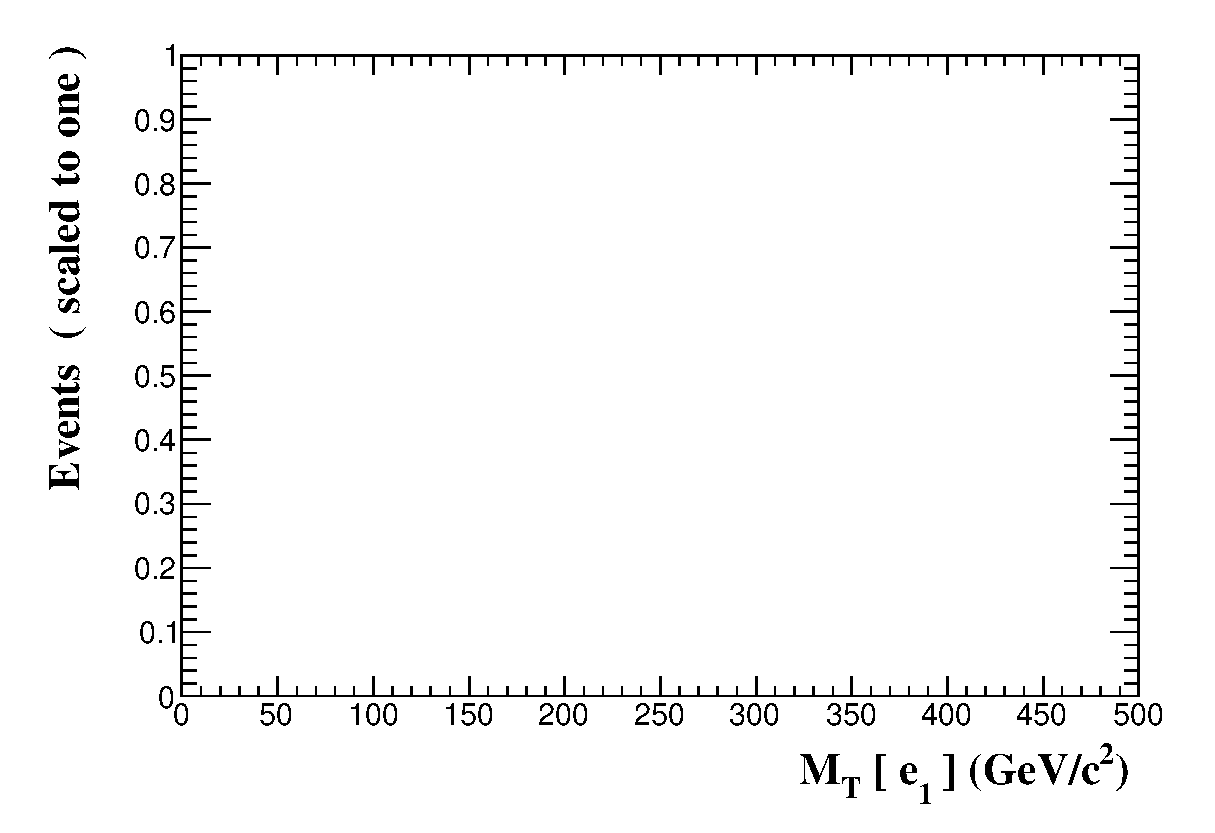
\includegraphics[scale=0.45]{selection_10.eps}\\
\caption{   }
  \end{center}
\end{figure}
      \newpage
\subsection{ Histogram 12}

\textbf{* Plot: PT ( mu[1] ) }\\
   \begin{table}[H]
  \begin{center}
    \begin{tabular}{|m{23.0mm}|m{23.0mm}|m{18.0mm}|m{19.0mm}|m{19.0mm}|m{19.0mm}|m{19.0mm}|}
      \hline
      {\cellcolor{yellow}         Dataset}& {\cellcolor{yellow}         Integral}& {\cellcolor{yellow}         Entries per event}& {\cellcolor{yellow}         Mean}& {\cellcolor{yellow}         RMS}& {\cellcolor{yellow}         \% underflow}& {\cellcolor{yellow}         \% overflow}\\
      \hline
      {\cellcolor{white}         tag\_1\_pythia8\_basicreco}& {\cellcolor{white}         0.0 +/\-- 0.0}& {\cellcolor{white}         1.0}& {\cellcolor{white}         0.0}& {\cellcolor{white}         0.0}& {\cellcolor{green}         0.0}& {\cellcolor{green}         0.0}\\
\hline
    \end{tabular}
  \end{center}
\end{table}

\begin{figure}[H]
  \begin{center}
    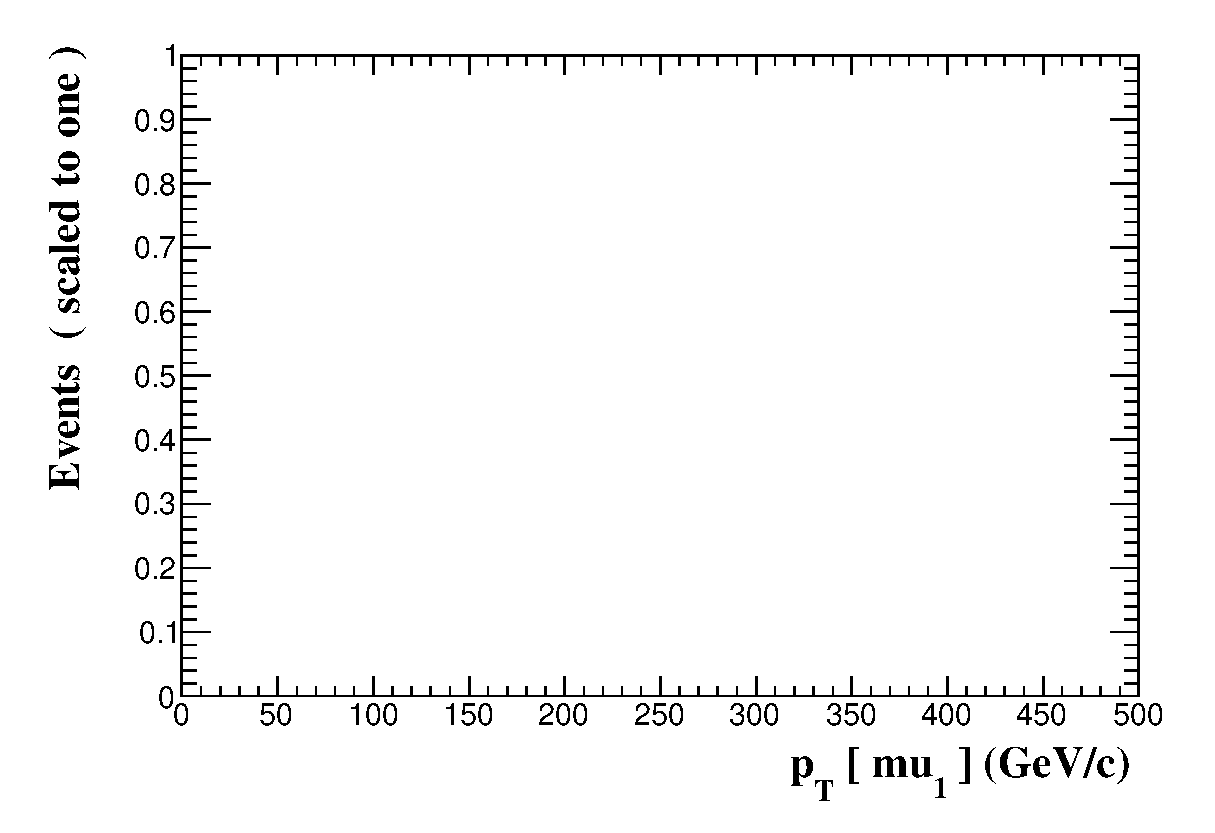
\includegraphics[scale=0.45]{selection_11.eps}\\
\caption{   }
  \end{center}
\end{figure}
      \newpage
\subsection{ Histogram 13}

\textbf{* Plot: ETA ( mu[1] ) }\\
   \begin{table}[H]
  \begin{center}
    \begin{tabular}{|m{23.0mm}|m{23.0mm}|m{18.0mm}|m{19.0mm}|m{19.0mm}|m{19.0mm}|m{19.0mm}|}
      \hline
      {\cellcolor{yellow}         Dataset}& {\cellcolor{yellow}         Integral}& {\cellcolor{yellow}         Entries per event}& {\cellcolor{yellow}         Mean}& {\cellcolor{yellow}         RMS}& {\cellcolor{yellow}         \% underflow}& {\cellcolor{yellow}         \% overflow}\\
      \hline
      {\cellcolor{white}         tag\_1\_pythia8\_basicreco}& {\cellcolor{white}         0.0 +/\-- 0.0}& {\cellcolor{white}         1.0}& {\cellcolor{white}         0.0}& {\cellcolor{white}         0.0}& {\cellcolor{green}         0.0}& {\cellcolor{green}         0.0}\\
\hline
    \end{tabular}
  \end{center}
\end{table}

\begin{figure}[H]
  \begin{center}
    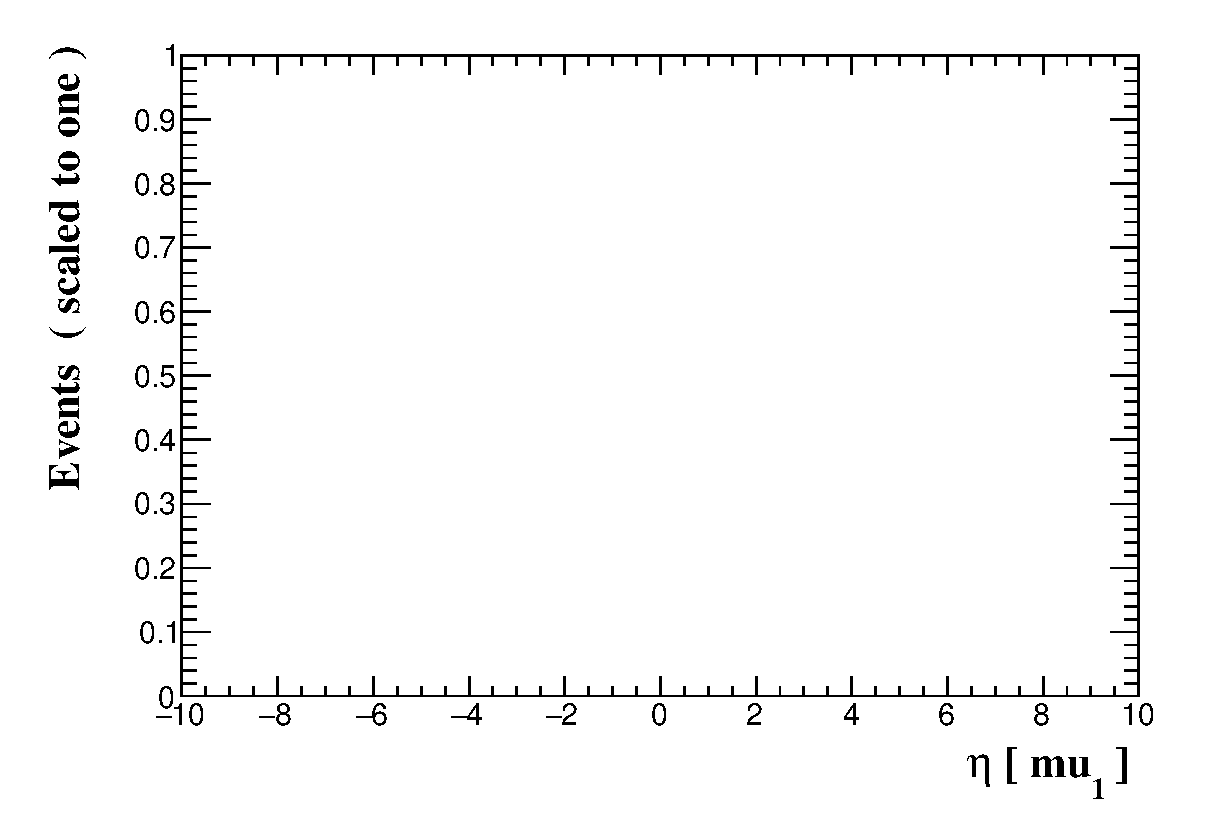
\includegraphics[scale=0.45]{selection_12.eps}\\
\caption{   }
  \end{center}
\end{figure}
      \newpage
\subsection{ Histogram 14}

\textbf{* Plot: MT\_MET ( mu[1] ) }\\
   \begin{table}[H]
  \begin{center}
    \begin{tabular}{|m{23.0mm}|m{23.0mm}|m{18.0mm}|m{19.0mm}|m{19.0mm}|m{19.0mm}|m{19.0mm}|}
      \hline
      {\cellcolor{yellow}         Dataset}& {\cellcolor{yellow}         Integral}& {\cellcolor{yellow}         Entries per event}& {\cellcolor{yellow}         Mean}& {\cellcolor{yellow}         RMS}& {\cellcolor{yellow}         \% underflow}& {\cellcolor{yellow}         \% overflow}\\
      \hline
      {\cellcolor{white}         tag\_1\_pythia8\_basicreco}& {\cellcolor{white}         0.0 +/\-- 0.0}& {\cellcolor{white}         1.0}& {\cellcolor{white}         0.0}& {\cellcolor{white}         0.0}& {\cellcolor{green}         0.0}& {\cellcolor{green}         0.0}\\
\hline
    \end{tabular}
  \end{center}
\end{table}

\begin{figure}[H]
  \begin{center}
    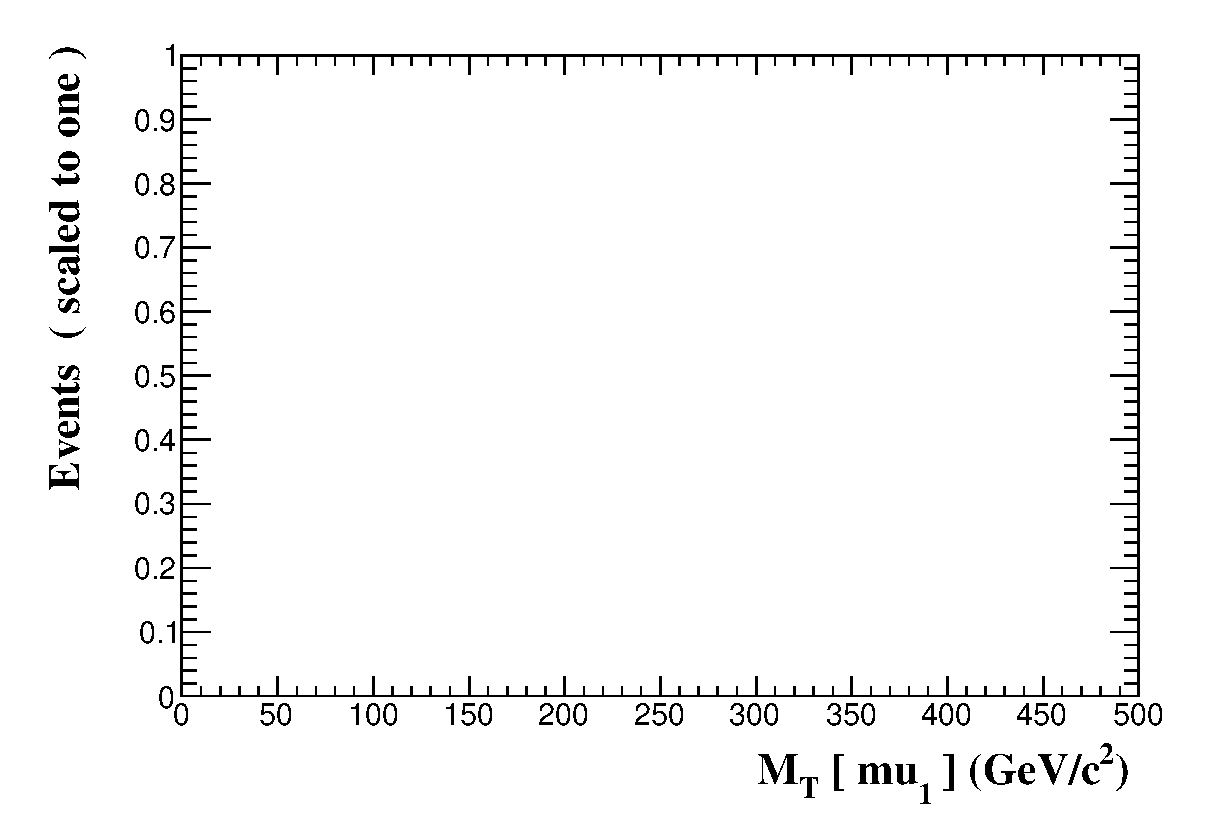
\includegraphics[scale=0.45]{selection_13.eps}\\
\caption{   }
  \end{center}
\end{figure}
      \newpage
\subsection{ Histogram 15}

\textbf{* Plot: M ( e[1] mu[1] ) }\\
   \begin{table}[H]
  \begin{center}
    \begin{tabular}{|m{23.0mm}|m{23.0mm}|m{18.0mm}|m{19.0mm}|m{19.0mm}|m{19.0mm}|m{19.0mm}|}
      \hline
      {\cellcolor{yellow}         Dataset}& {\cellcolor{yellow}         Integral}& {\cellcolor{yellow}         Entries per event}& {\cellcolor{yellow}         Mean}& {\cellcolor{yellow}         RMS}& {\cellcolor{yellow}         \% underflow}& {\cellcolor{yellow}         \% overflow}\\
      \hline
      {\cellcolor{white}         tag\_1\_pythia8\_basicreco}& {\cellcolor{white}         0.0 +/\-- 0.0}& {\cellcolor{white}         0.}& {\cellcolor{white}         0.0}& {\cellcolor{white}         0.0}& {\cellcolor{green}         0.0}& {\cellcolor{green}         0.0}\\
\hline
    \end{tabular}
  \end{center}
\end{table}

\begin{figure}[H]
  \begin{center}
    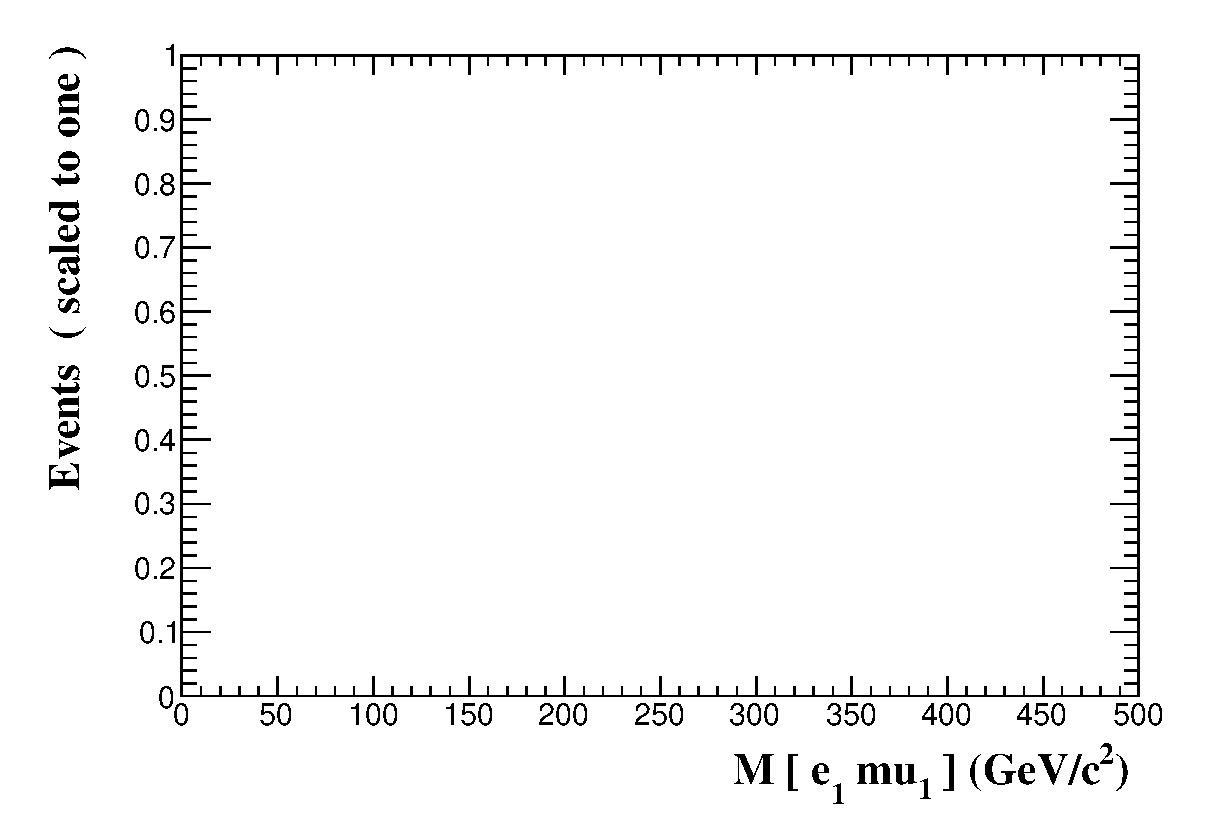
\includegraphics[scale=0.45]{selection_14.eps}\\
\caption{   }
  \end{center}
\end{figure}
      \newpage
\subsection{ Histogram 16}

\textbf{* Plot: M ( e[1] j[1] ) }\\
   \begin{table}[H]
  \begin{center}
    \begin{tabular}{|m{23.0mm}|m{23.0mm}|m{18.0mm}|m{19.0mm}|m{19.0mm}|m{19.0mm}|m{19.0mm}|}
      \hline
      {\cellcolor{yellow}         Dataset}& {\cellcolor{yellow}         Integral}& {\cellcolor{yellow}         Entries per event}& {\cellcolor{yellow}         Mean}& {\cellcolor{yellow}         RMS}& {\cellcolor{yellow}         \% underflow}& {\cellcolor{yellow}         \% overflow}\\
      \hline
      {\cellcolor{white}         tag\_1\_pythia8\_basicreco}& {\cellcolor{white}         0.0 +/\-- 0.0}& {\cellcolor{white}         1.0}& {\cellcolor{white}         0.0}& {\cellcolor{white}         0.0}& {\cellcolor{green}         0.0}& {\cellcolor{green}         0.0}\\
\hline
    \end{tabular}
  \end{center}
\end{table}

\begin{figure}[H]
  \begin{center}
    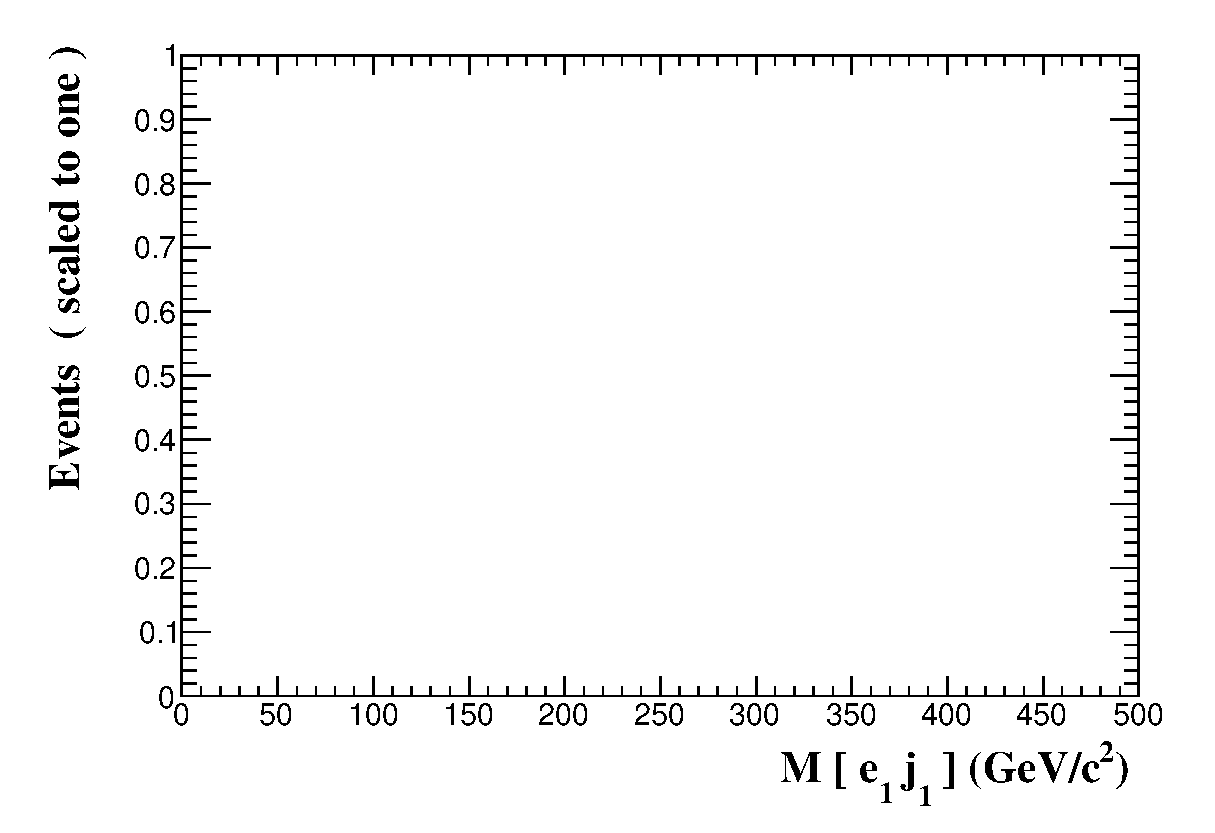
\includegraphics[scale=0.45]{selection_15.eps}\\
\caption{   }
  \end{center}
\end{figure}
      \newpage
\subsection{ Histogram 17}

\textbf{* Plot: M ( j[1] j[2] ) }\\
   \begin{table}[H]
  \begin{center}
    \begin{tabular}{|m{23.0mm}|m{23.0mm}|m{18.0mm}|m{19.0mm}|m{19.0mm}|m{19.0mm}|m{19.0mm}|}
      \hline
      {\cellcolor{yellow}         Dataset}& {\cellcolor{yellow}         Integral}& {\cellcolor{yellow}         Entries per event}& {\cellcolor{yellow}         Mean}& {\cellcolor{yellow}         RMS}& {\cellcolor{yellow}         \% underflow}& {\cellcolor{yellow}         \% overflow}\\
      \hline
      {\cellcolor{white}         tag\_1\_pythia8\_basicreco}& {\cellcolor{white}         0.0 +/\-- 0.0}& {\cellcolor{white}         1.0}& {\cellcolor{white}         0.0}& {\cellcolor{white}         0.0}& {\cellcolor{green}         0.0}& {\cellcolor{green}         0.0}\\
\hline
    \end{tabular}
  \end{center}
\end{table}

\begin{figure}[H]
  \begin{center}
    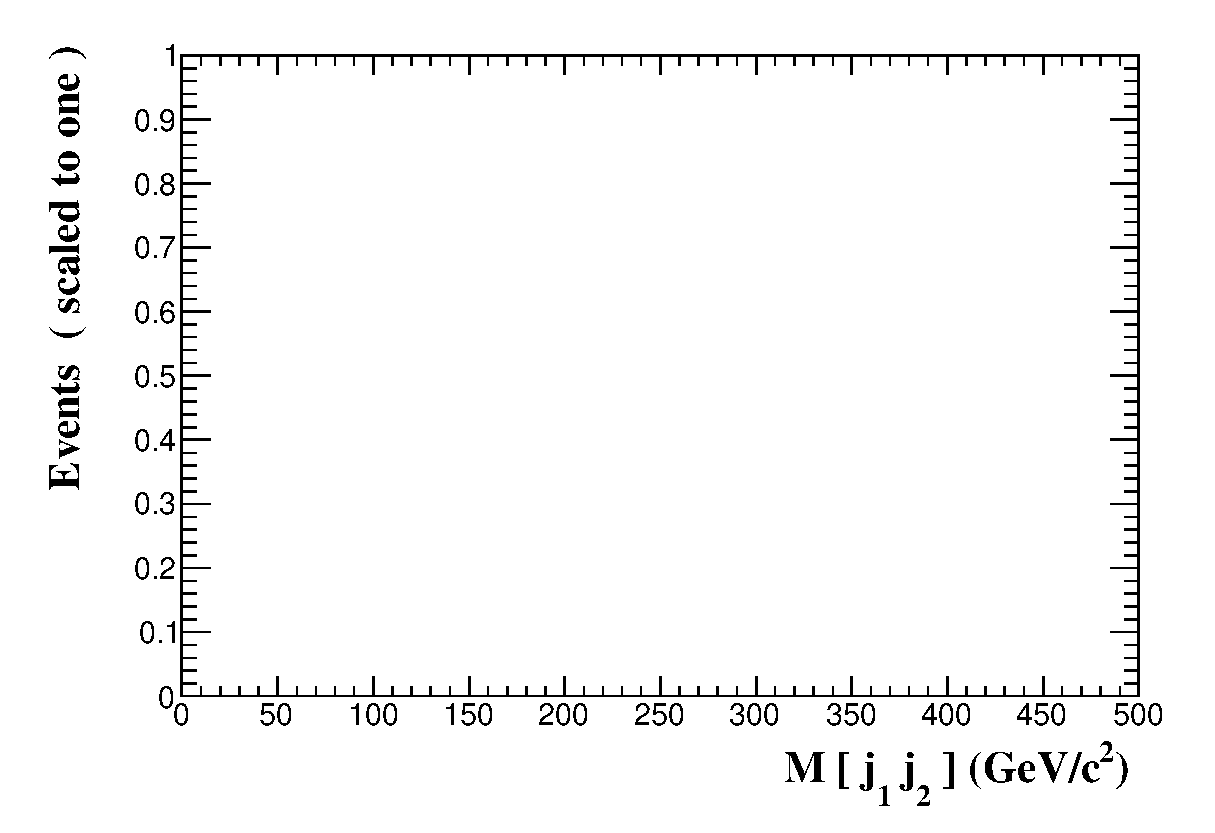
\includegraphics[scale=0.45]{selection_16.eps}\\
\caption{   }
  \end{center}
\end{figure}
      \newpage
\subsection{ Histogram 18}

\textbf{* Plot: M ( j[1] mu[1] ) }\\
   \begin{table}[H]
  \begin{center}
    \begin{tabular}{|m{23.0mm}|m{23.0mm}|m{18.0mm}|m{19.0mm}|m{19.0mm}|m{19.0mm}|m{19.0mm}|}
      \hline
      {\cellcolor{yellow}         Dataset}& {\cellcolor{yellow}         Integral}& {\cellcolor{yellow}         Entries per event}& {\cellcolor{yellow}         Mean}& {\cellcolor{yellow}         RMS}& {\cellcolor{yellow}         \% underflow}& {\cellcolor{yellow}         \% overflow}\\
      \hline
      {\cellcolor{white}         tag\_1\_pythia8\_basicreco}& {\cellcolor{white}         0.0 +/\-- 0.0}& {\cellcolor{white}         1.0}& {\cellcolor{white}         0.0}& {\cellcolor{white}         0.0}& {\cellcolor{green}         0.0}& {\cellcolor{green}         0.0}\\
\hline
    \end{tabular}
  \end{center}
\end{table}

\begin{figure}[H]
  \begin{center}
    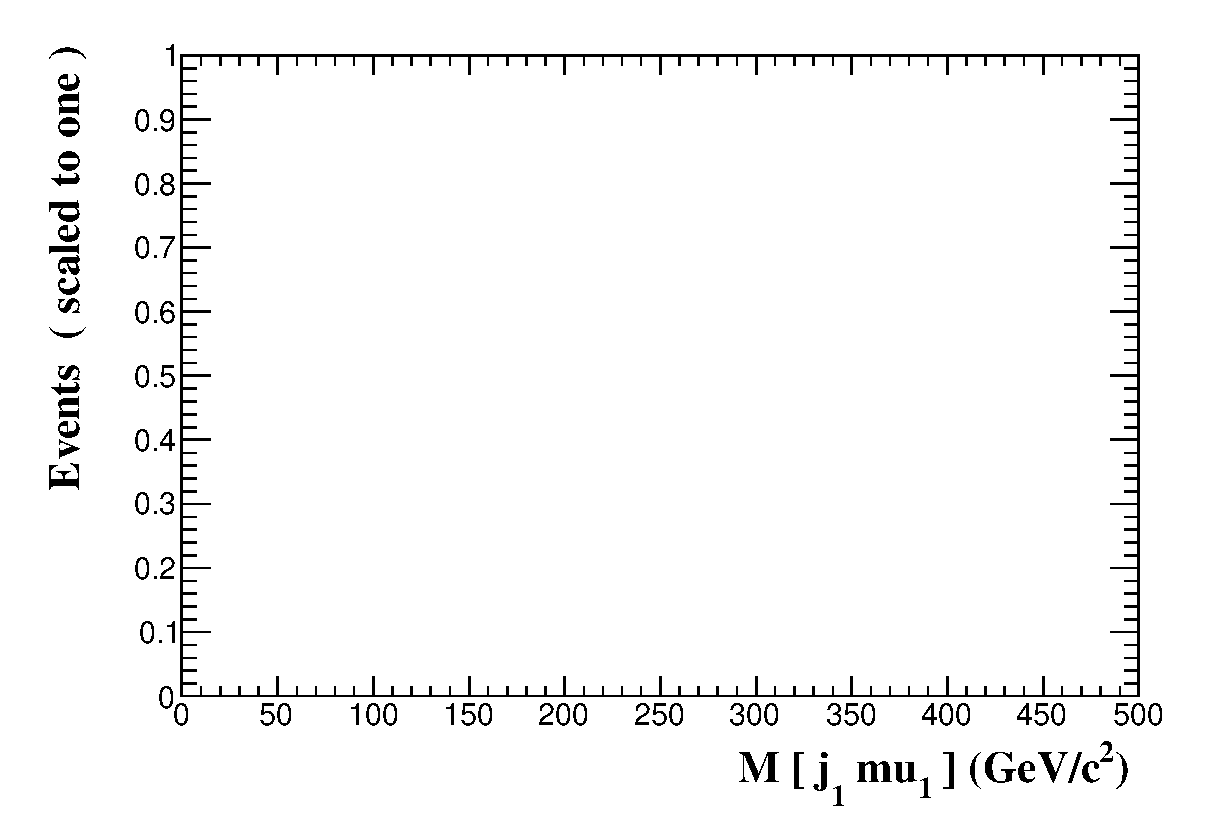
\includegraphics[scale=0.45]{selection_17.eps}\\
\caption{   }
  \end{center}
\end{figure}
      \newpage
\subsection{ Histogram 19}

\textbf{* Plot: M ( e[1] j[2] ) }\\
   \begin{table}[H]
  \begin{center}
    \begin{tabular}{|m{23.0mm}|m{23.0mm}|m{18.0mm}|m{19.0mm}|m{19.0mm}|m{19.0mm}|m{19.0mm}|}
      \hline
      {\cellcolor{yellow}         Dataset}& {\cellcolor{yellow}         Integral}& {\cellcolor{yellow}         Entries per event}& {\cellcolor{yellow}         Mean}& {\cellcolor{yellow}         RMS}& {\cellcolor{yellow}         \% underflow}& {\cellcolor{yellow}         \% overflow}\\
      \hline
      {\cellcolor{white}         tag\_1\_pythia8\_basicreco}& {\cellcolor{white}         0.0 +/\-- 0.0}& {\cellcolor{white}         1.0}& {\cellcolor{white}         0.0}& {\cellcolor{white}         0.0}& {\cellcolor{green}         0.0}& {\cellcolor{green}         0.0}\\
\hline
    \end{tabular}
  \end{center}
\end{table}

\begin{figure}[H]
  \begin{center}
    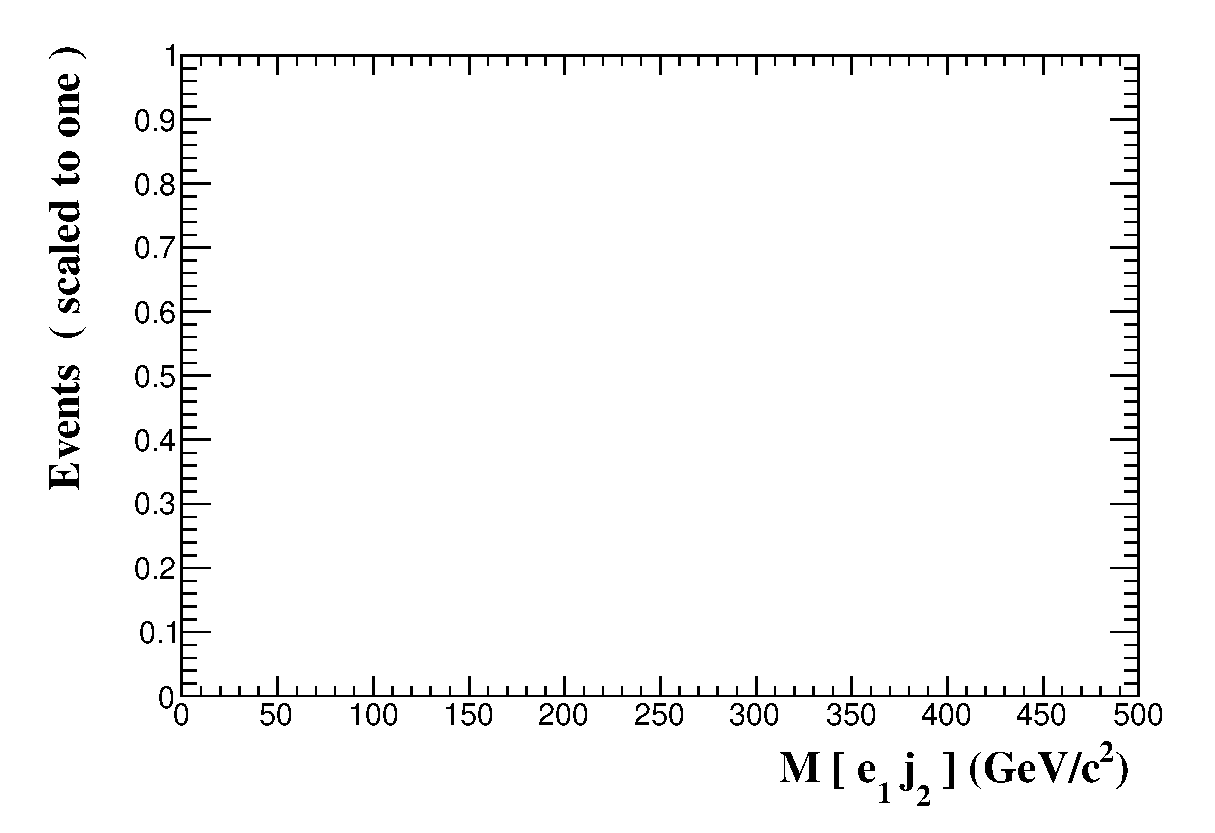
\includegraphics[scale=0.45]{selection_18.eps}\\
\caption{   }
  \end{center}
\end{figure}
      \newpage
\subsection{ Histogram 20}

\textbf{* Plot: M ( j[2] mu[1] ) }\\
   \begin{table}[H]
  \begin{center}
    \begin{tabular}{|m{23.0mm}|m{23.0mm}|m{18.0mm}|m{19.0mm}|m{19.0mm}|m{19.0mm}|m{19.0mm}|}
      \hline
      {\cellcolor{yellow}         Dataset}& {\cellcolor{yellow}         Integral}& {\cellcolor{yellow}         Entries per event}& {\cellcolor{yellow}         Mean}& {\cellcolor{yellow}         RMS}& {\cellcolor{yellow}         \% underflow}& {\cellcolor{yellow}         \% overflow}\\
      \hline
      {\cellcolor{white}         tag\_1\_pythia8\_basicreco}& {\cellcolor{white}         0.0 +/\-- 0.0}& {\cellcolor{white}         1.0}& {\cellcolor{white}         0.0}& {\cellcolor{white}         0.0}& {\cellcolor{green}         0.0}& {\cellcolor{green}         0.0}\\
\hline
    \end{tabular}
  \end{center}
\end{table}

\begin{figure}[H]
  \begin{center}
    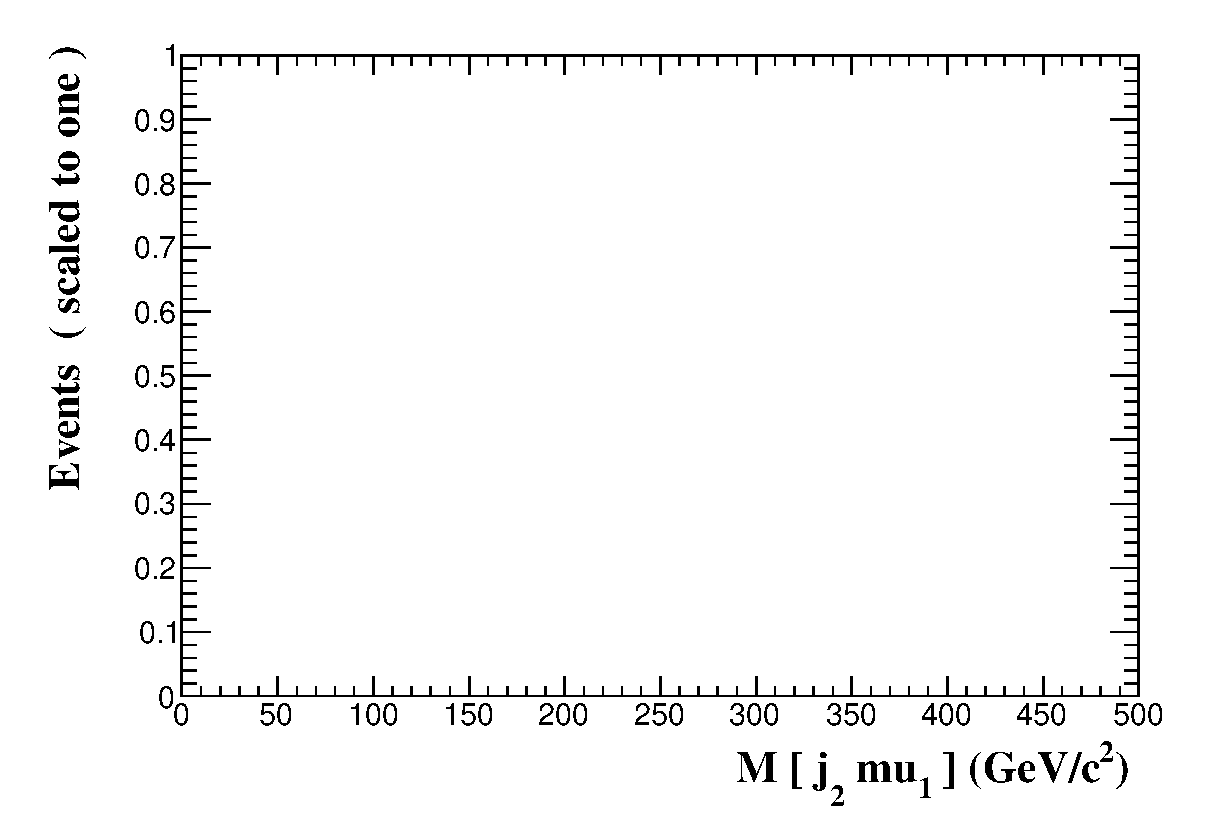
\includegraphics[scale=0.45]{selection_19.eps}\\
\caption{   }
  \end{center}
\end{figure}
      \newpage
\subsection{ Histogram 21}

\textbf{* Plot: DELTAR ( e[1] , mu[1] ) }\\
   \begin{table}[H]
  \begin{center}
    \begin{tabular}{|m{23.0mm}|m{23.0mm}|m{18.0mm}|m{19.0mm}|m{19.0mm}|m{19.0mm}|m{19.0mm}|}
      \hline
      {\cellcolor{yellow}         Dataset}& {\cellcolor{yellow}         Integral}& {\cellcolor{yellow}         Entries per event}& {\cellcolor{yellow}         Mean}& {\cellcolor{yellow}         RMS}& {\cellcolor{yellow}         \% underflow}& {\cellcolor{yellow}         \% overflow}\\
      \hline
      {\cellcolor{white}         tag\_1\_pythia8\_basicreco}& {\cellcolor{white}         0.0 +/\-- 0.0}& {\cellcolor{white}         0.}& {\cellcolor{white}         0.0}& {\cellcolor{white}         0.0}& {\cellcolor{green}         0.0}& {\cellcolor{green}         0.0}\\
\hline
    \end{tabular}
  \end{center}
\end{table}

\begin{figure}[H]
  \begin{center}
    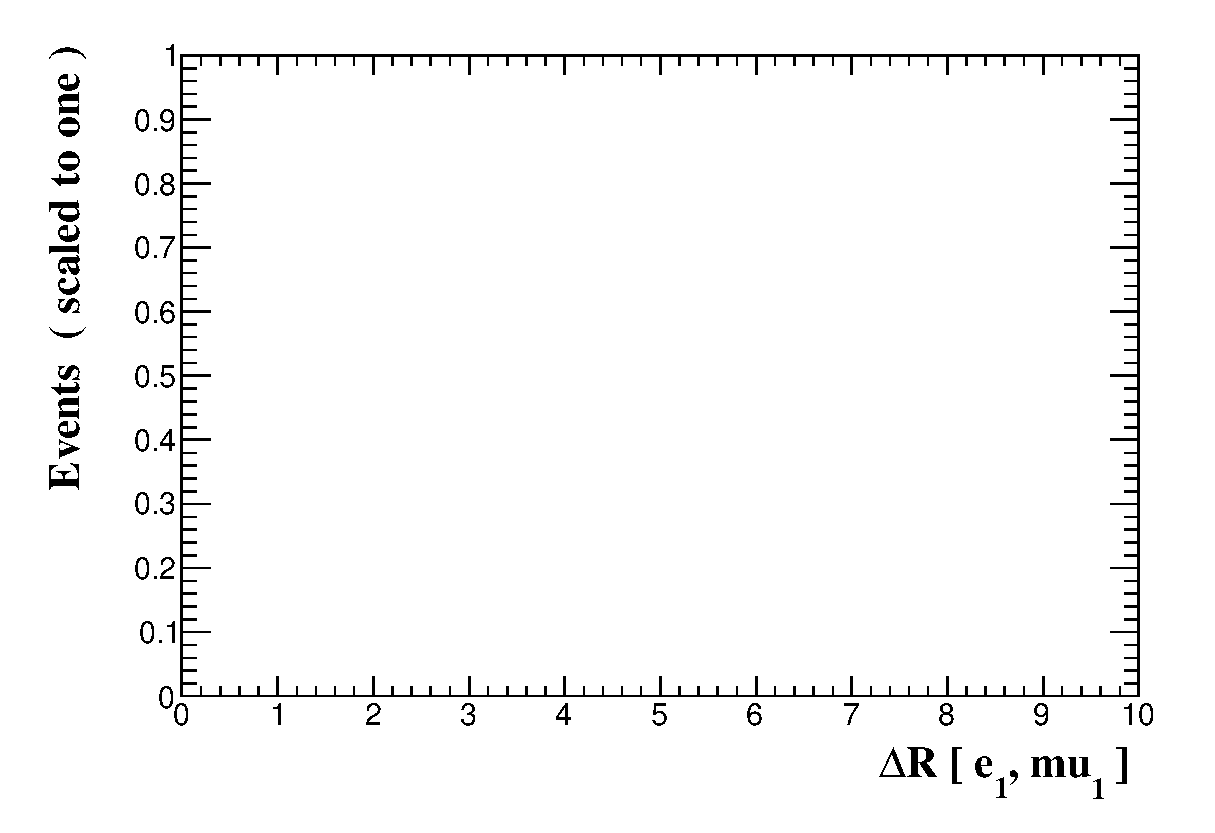
\includegraphics[scale=0.45]{selection_20.eps}\\
\caption{   }
  \end{center}
\end{figure}
      \newpage
\subsection{ Histogram 22}

\textbf{* Plot: DELTAR ( j[1] , e[1] ) }\\
   \begin{table}[H]
  \begin{center}
    \begin{tabular}{|m{23.0mm}|m{23.0mm}|m{18.0mm}|m{19.0mm}|m{19.0mm}|m{19.0mm}|m{19.0mm}|}
      \hline
      {\cellcolor{yellow}         Dataset}& {\cellcolor{yellow}         Integral}& {\cellcolor{yellow}         Entries per event}& {\cellcolor{yellow}         Mean}& {\cellcolor{yellow}         RMS}& {\cellcolor{yellow}         \% underflow}& {\cellcolor{yellow}         \% overflow}\\
      \hline
      {\cellcolor{white}         tag\_1\_pythia8\_basicreco}& {\cellcolor{white}         0.0 +/\-- 0.0}& {\cellcolor{white}         1.0}& {\cellcolor{white}         0.0}& {\cellcolor{white}         0.0}& {\cellcolor{green}         0.0}& {\cellcolor{green}         0.0}\\
\hline
    \end{tabular}
  \end{center}
\end{table}

\begin{figure}[H]
  \begin{center}
    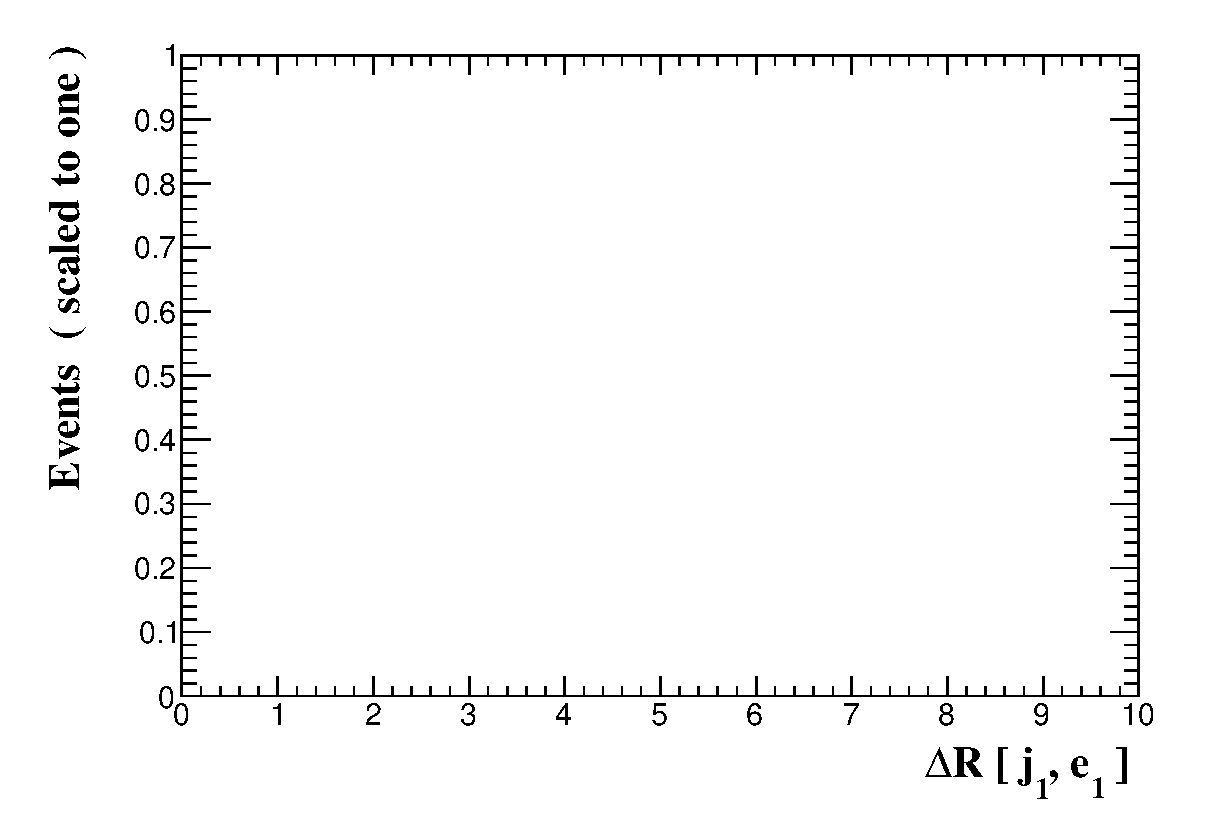
\includegraphics[scale=0.45]{selection_21.eps}\\
\caption{   }
  \end{center}
\end{figure}
      \newpage
\subsection{ Histogram 23}

\textbf{* Plot: DELTAR ( j[1] , j[2] ) }\\
   \begin{table}[H]
  \begin{center}
    \begin{tabular}{|m{23.0mm}|m{23.0mm}|m{18.0mm}|m{19.0mm}|m{19.0mm}|m{19.0mm}|m{19.0mm}|}
      \hline
      {\cellcolor{yellow}         Dataset}& {\cellcolor{yellow}         Integral}& {\cellcolor{yellow}         Entries per event}& {\cellcolor{yellow}         Mean}& {\cellcolor{yellow}         RMS}& {\cellcolor{yellow}         \% underflow}& {\cellcolor{yellow}         \% overflow}\\
      \hline
      {\cellcolor{white}         tag\_1\_pythia8\_basicreco}& {\cellcolor{white}         0.0 +/\-- 0.0}& {\cellcolor{white}         1.0}& {\cellcolor{white}         0.0}& {\cellcolor{white}         0.0}& {\cellcolor{green}         0.0}& {\cellcolor{green}         0.0}\\
\hline
    \end{tabular}
  \end{center}
\end{table}

\begin{figure}[H]
  \begin{center}
    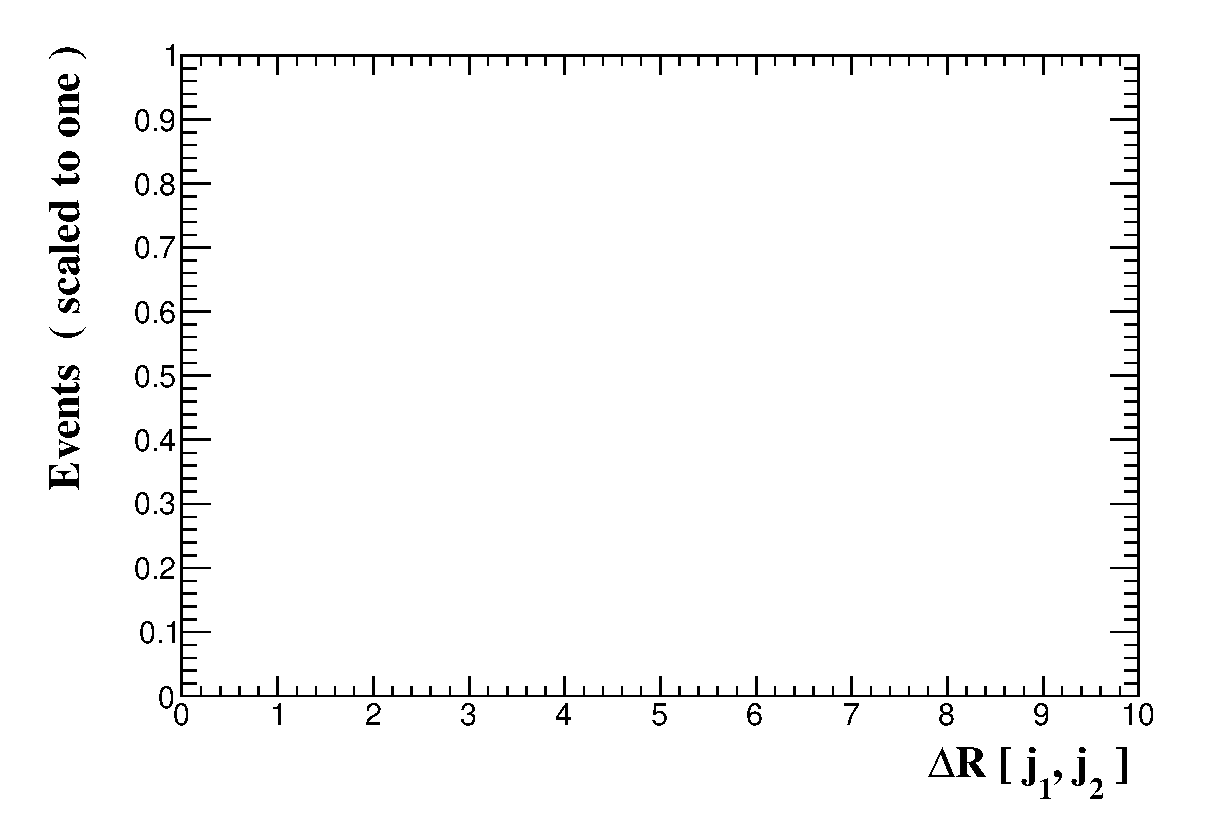
\includegraphics[scale=0.45]{selection_22.eps}\\
\caption{   }
  \end{center}
\end{figure}
      \newpage
\subsection{ Histogram 24}

\textbf{* Plot: DELTAR ( j[1] , mu[1] ) }\\
   \begin{table}[H]
  \begin{center}
    \begin{tabular}{|m{23.0mm}|m{23.0mm}|m{18.0mm}|m{19.0mm}|m{19.0mm}|m{19.0mm}|m{19.0mm}|}
      \hline
      {\cellcolor{yellow}         Dataset}& {\cellcolor{yellow}         Integral}& {\cellcolor{yellow}         Entries per event}& {\cellcolor{yellow}         Mean}& {\cellcolor{yellow}         RMS}& {\cellcolor{yellow}         \% underflow}& {\cellcolor{yellow}         \% overflow}\\
      \hline
      {\cellcolor{white}         tag\_1\_pythia8\_basicreco}& {\cellcolor{white}         0.0 +/\-- 0.0}& {\cellcolor{white}         1.0}& {\cellcolor{white}         0.0}& {\cellcolor{white}         0.0}& {\cellcolor{green}         0.0}& {\cellcolor{green}         0.0}\\
\hline
    \end{tabular}
  \end{center}
\end{table}

\begin{figure}[H]
  \begin{center}
    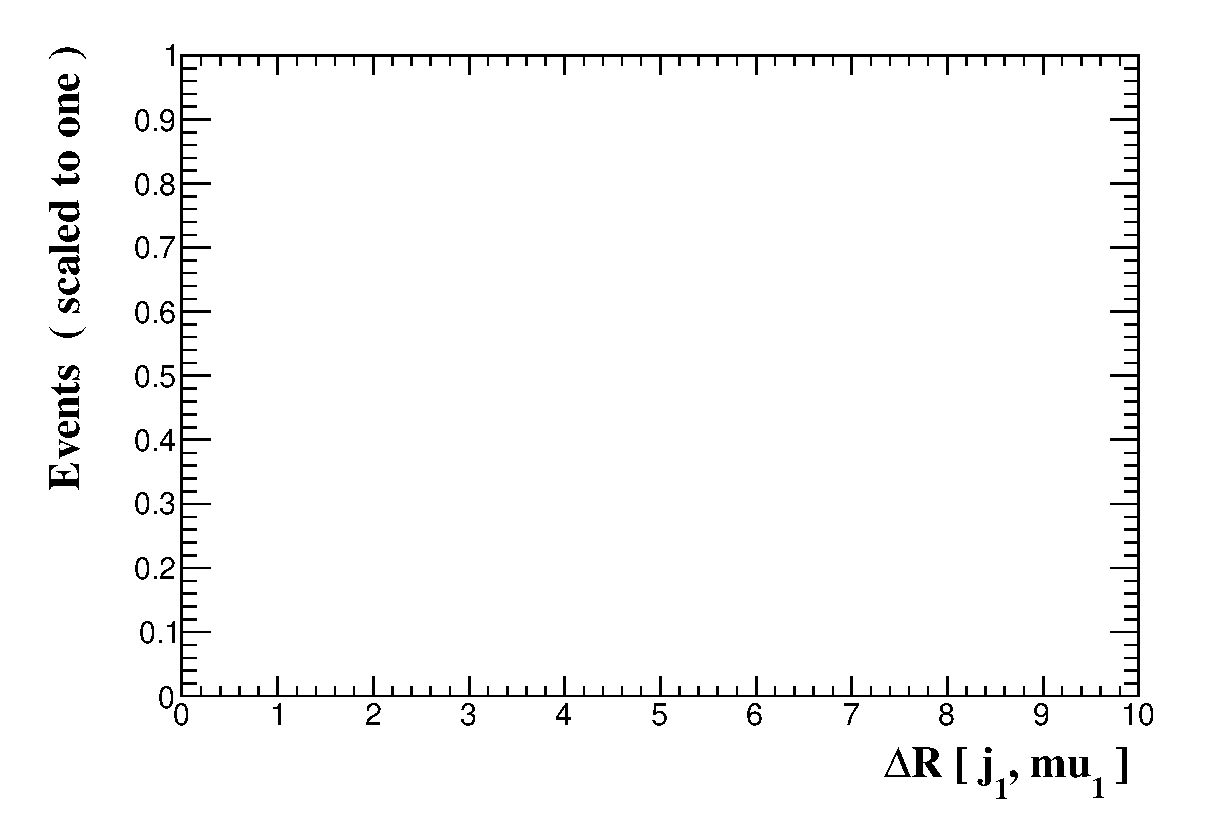
\includegraphics[scale=0.45]{selection_23.eps}\\
\caption{   }
  \end{center}
\end{figure}
      \newpage
\subsection{ Histogram 25}

\textbf{* Plot: DELTAR ( j[2] , e[1] ) }\\
   \begin{table}[H]
  \begin{center}
    \begin{tabular}{|m{23.0mm}|m{23.0mm}|m{18.0mm}|m{19.0mm}|m{19.0mm}|m{19.0mm}|m{19.0mm}|}
      \hline
      {\cellcolor{yellow}         Dataset}& {\cellcolor{yellow}         Integral}& {\cellcolor{yellow}         Entries per event}& {\cellcolor{yellow}         Mean}& {\cellcolor{yellow}         RMS}& {\cellcolor{yellow}         \% underflow}& {\cellcolor{yellow}         \% overflow}\\
      \hline
      {\cellcolor{white}         tag\_1\_pythia8\_basicreco}& {\cellcolor{white}         0.0 +/\-- 0.0}& {\cellcolor{white}         1.0}& {\cellcolor{white}         0.0}& {\cellcolor{white}         0.0}& {\cellcolor{green}         0.0}& {\cellcolor{green}         0.0}\\
\hline
    \end{tabular}
  \end{center}
\end{table}

\begin{figure}[H]
  \begin{center}
    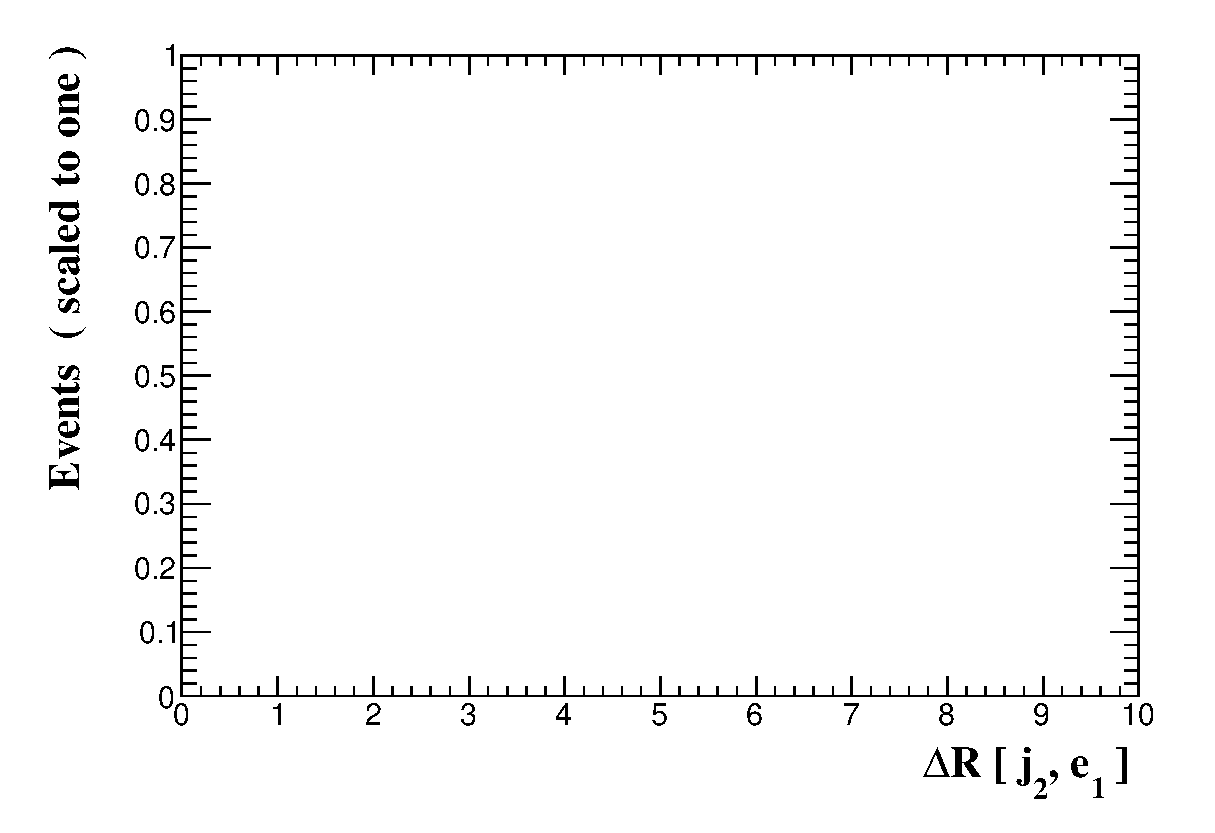
\includegraphics[scale=0.45]{selection_24.eps}\\
\caption{   }
  \end{center}
\end{figure}
      \newpage
\subsection{ Histogram 26}

\textbf{* Plot: DELTAR ( j[2] , mu[1] ) }\\
   \begin{table}[H]
  \begin{center}
    \begin{tabular}{|m{23.0mm}|m{23.0mm}|m{18.0mm}|m{19.0mm}|m{19.0mm}|m{19.0mm}|m{19.0mm}|}
      \hline
      {\cellcolor{yellow}         Dataset}& {\cellcolor{yellow}         Integral}& {\cellcolor{yellow}         Entries per event}& {\cellcolor{yellow}         Mean}& {\cellcolor{yellow}         RMS}& {\cellcolor{yellow}         \% underflow}& {\cellcolor{yellow}         \% overflow}\\
      \hline
      {\cellcolor{white}         tag\_1\_pythia8\_basicreco}& {\cellcolor{white}         0.0 +/\-- 0.0}& {\cellcolor{white}         1.0}& {\cellcolor{white}         0.0}& {\cellcolor{white}         0.0}& {\cellcolor{green}         0.0}& {\cellcolor{green}         0.0}\\
\hline
    \end{tabular}
  \end{center}
\end{table}

\begin{figure}[H]
  \begin{center}
    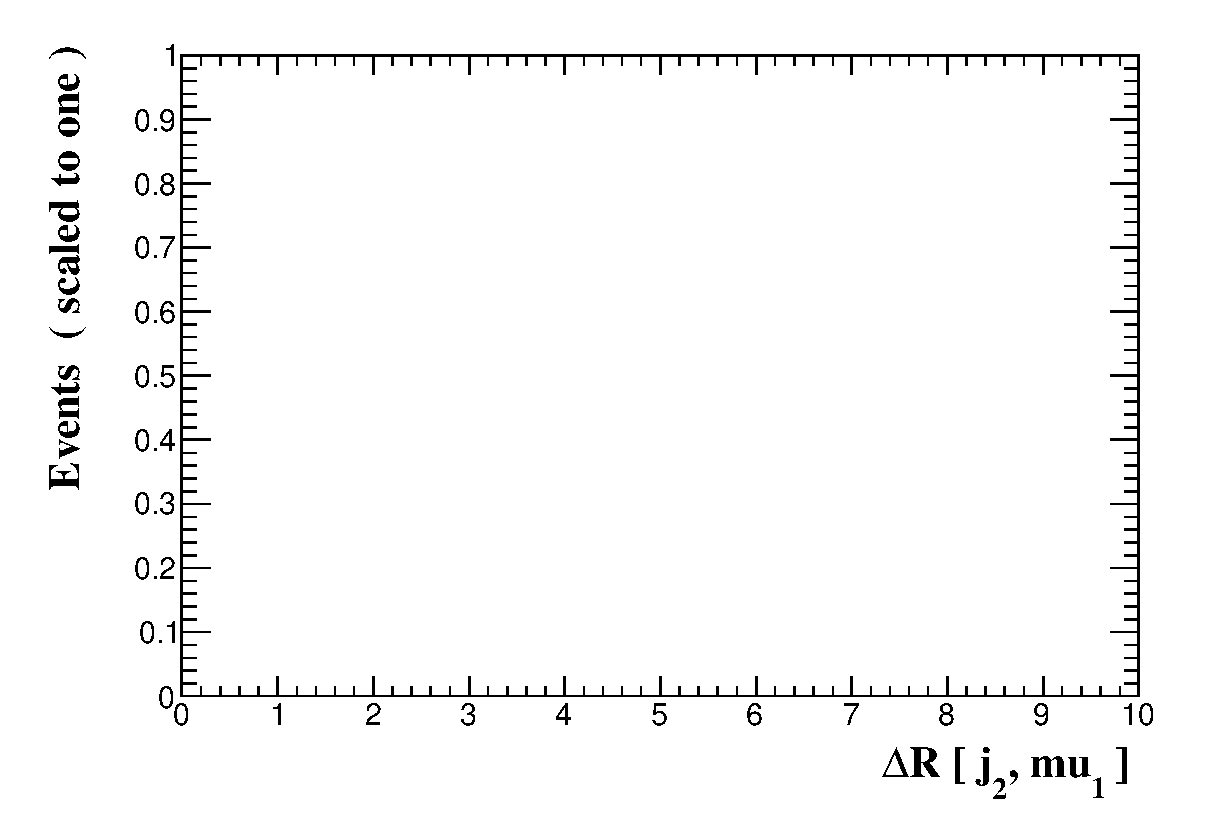
\includegraphics[scale=0.45]{selection_25.eps}\\
\caption{   }
  \end{center}
\end{figure}
      % -----------------------------------------------------------------------------
%                                SECTION Summary                                
% -----------------------------------------------------------------------------
\newpage
\section{ Summary}

\subsection{Cut-flow charts}

\begin{itemize}
  \item How to compare signal (S) and background (B): \textcolor{blue}{S/\-sqrt(S+B)} .
   \item Object definition selections are indicated in cyan.  \item Reject and select are indicated by 'REJ' and 'SEL' respectively
\end{itemize}
\begin{table}[H]
  \begin{center}
    \begin{tabular}{|m{36.0mm}|m{36.0mm}|m{36.0mm}|m{33.0mm}|}
      \hline
      {\cellcolor{yellow}        Cuts}& {\cellcolor{yellow}         Signal (S)}& {\cellcolor{yellow}         Background (B)}& {\cellcolor{yellow}         S vs B}\\
      \hline
      {\cellcolor{white}         Initial (no cut)}& {\cellcolor{white}         0.0 +/\-- 0.0}& {\cellcolor{white}         }& {\cellcolor{white}         }\\
\hline
    \end{tabular}
  \end{center}
\end{table}

\end{document}
